% ==================================================================
% TEMPLATE TCC MACKENZIE - BRUNO GASPARONI BALLERINI
% Baseado nas normas do Guia do TCC 2022 - Universidade Presbiteriana Mackenzie
% ==================================================================

\documentclass[12pt,a4paper,oneside]{report}

% ==================================================================
% PACOTES NECESSÁRIOS
% ==================================================================
\usepackage[utf8]{inputenc}
\usepackage[T1]{fontenc}
\usepackage[portuguese]{babel}
\usepackage{mathptmx} % Times New Roman
\usepackage{setspace}
\usepackage{geometry}
\usepackage{titlesec}
\usepackage{tocloft}
\usepackage{fancyhdr}
\usepackage{graphicx}
\usepackage{amsmath}
\usepackage{amsfonts}
\usepackage{amssymb}
\usepackage{indentfirst}
\usepackage{caption}
\usepackage{subcaption}
\usepackage{float}
\usepackage[hidelinks]{hyperref}
\usepackage{url}
\usepackage{booktabs}
\usepackage{xcolor}
\usepackage{array}
\usepackage{multirow}
\usepackage{longtable}

% ==================================================================
% CONFIGURAÇÕES GERAIS MACKENZIE
% ==================================================================

% Margens: 3cm (superior e esquerda), 2cm (inferior e direita)
\geometry{
    a4paper,
    top=3cm,
    left=3cm,
    bottom=2cm,
    right=2cm
}

% Espaçamento 1.5
\onehalfspacing

% Recuo de parágrafo 1,25cm
\setlength{\parindent}{1.25cm}

% Espaçamento entre parágrafos - SEM espaço extra (conforme guia p.40)
\setlength{\parskip}{0pt}

% ==================================================================
% CONFIGURAÇÃO DE TÍTULOS (NORMAS MACKENZIE)
% ==================================================================

% Seção primária: 1 LETRAS MAIÚSCULAS EM NEGRITO  
\titleformat{\chapter}[hang]
{\normalfont\fontsize{12}{14.4}\bfseries}
{\thechapter}{1em}{\MakeUppercase}
\titlespacing*{\chapter}{0pt}{0pt}{12pt}

% Títulos de capítulos não numerados (centralizados)
\titleformat{name=\chapter,numberless}[block]
{\normalfont\fontsize{12}{14.4}\bfseries\centering}
{}{0pt}{\MakeUppercase}
\titlespacing*{name=\chapter,numberless}{0pt}{0pt}{12pt}

% Seção secundária: 1.1 LETRAS MAIÚSCULAS SEM NEGRITO
\titleformat{\section}[hang]
{\normalfont\fontsize{12}{14.4}}
{\thesection}{1em}{\MakeUppercase}
\titlespacing*{\section}{0pt}{\baselineskip}{\baselineskip}

% Seção terciária: 1.1.1 Letras minúsculas em negrito
\titleformat{\subsection}[hang]
{\normalfont\fontsize{12}{14.4}\bfseries}
{\thesubsection}{1em}{}
\titlespacing*{\subsection}{0pt}{12pt}{12pt}

% Seção quaternária: 1.1.1.1 Letras minúsculas sem negrito
\titleformat{\subsubsection}[hang]
{\normalfont\fontsize{12}{14.4}}
{\thesubsubsection}{1em}{}
\titlespacing*{\subsubsection}{0pt}{12pt}{12pt}

% Seção quinária: 1.1.1.1.1 Letras minúsculas em itálico
\titleformat{\paragraph}[hang]
{\normalfont\fontsize{12}{14.4}\itshape}
{\theparagraph}{1em}{}
\titlespacing*{\paragraph}{0pt}{12pt}{12pt}

% ==================================================================
% CONFIGURAÇÃO DE NUMERAÇÃO
% ==================================================================

% Numeração sequencial simples para equações (sem capítulo)
\renewcommand{\theequation}{\arabic{equation}}

% ==================================================================
% NUMERAÇÃO DE PÁGINAS
% ==================================================================
\setlength{\headheight}{13.19998pt}
\pagestyle{fancy}
\fancyhf{}
% Numeração a 2cm das bordas superior e direita
\fancyhead[R]{\fontsize{11}{13.2}\selectfont\thepage}
\fancyheadoffset{0cm}
\renewcommand{\headrulewidth}{0pt}

% ==================================================================
% CONFIGURAÇÃO DO SUMÁRIO
% ==================================================================
\renewcommand{\contentsname}{SUMÁRIO}
\renewcommand{\cftchapfont}{\fontsize{12}{14.4}\selectfont\bfseries}
\renewcommand{\cftsecfont}{\fontsize{12}{14.4}\selectfont}
\renewcommand{\cftsubsecfont}{\fontsize{12}{14.4}\selectfont}
\renewcommand{\cftchapleader}{\cftdotfill{\cftdotsep}}
\setlength{\cftbeforechapskip}{3pt}
\setlength{\cftbeforesecskip}{1pt}
\setlength{\cftbeforesubsecskip}{1pt}
% Limitar profundidade do sumário a 3 níveis
\setcounter{tocdepth}{3}

% ==================================================================
% INÍCIO DO DOCUMENTO
% ==================================================================
\begin{document}

% CAPA - sem numeração
\pagenumbering{gobble}
% ==================================================================
% CAPA - CONFORME MODELO MACKENZIE (Apêndice D do Guia)
% ==================================================================

\thispagestyle{empty}

\begin{center}

% Espaçamento superior
\vspace*{3cm}

% Nome da instituição
{\fontsize{12}{14.4}\selectfont\bfseries\MakeUppercase{UNIVERSIDADE PRESBITERIANA MACKENZIE}}\\[0.8cm]
{\fontsize{12}{14.4}\selectfont\bfseries\MakeUppercase{Centro de Ciências e Tecnologia – CCT}}\\[0.5cm]
{\fontsize{12}{14.4}\selectfont\bfseries\MakeUppercase{Curso de Engenharia de Produção}}

\vspace{5cm}

% Nome do autor
{\fontsize{12}{14.4}\selectfont\bfseries\MakeUppercase{BRUNO GASPARONI BALLERINI}}

\vspace{5cm}

% Título do trabalho
{\fontsize{12}{14.4}\selectfont\bfseries\MakeUppercase{%
COMPARAÇÃO ENTRE MÉTODOS DE ALOCAÇÃO DE CARTEIRAS:\\[0.3cm]
MARKOWITZ, EQUAL WEIGHT E RISK PARITY\\[0.3cm] 
NO MERCADO BRASILEIRO (2018–2019)%
}}

\vfill

% Local e ano
{\fontsize{12}{14.4}\selectfont
Campinas\\[0.3cm]
2025}

\end{center}
\newpage

% FOLHA DE ROSTO - inicia contagem (página 1, mas não aparece)
\pagenumbering{arabic}
\setcounter{page}{1}
\thispagestyle{empty}
% ==================================================================
% FOLHA DE ROSTO - CONFORME MODELO MACKENZIE (Apêndice E do Guia)
% ==================================================================

\thispagestyle{empty}

\begin{center}

\vspace*{2cm}

% Nome do autor
{\fontsize{12}{14.4}\selectfont\MakeUppercase{BRUNO GASPARONI BALLERINI}}\\[0.3cm]
{\fontsize{12}{14.4}\selectfont RA: 10387933}

\vspace{4cm}

% Título do trabalho
{\fontsize{12}{14.4}\selectfont\MakeUppercase{%
COMPARAÇÃO ENTRE MÉTODOS DE ALOCAÇÃO DE CARTEIRAS:\\[0.3cm]
MARKOWITZ, EQUAL WEIGHT E RISK PARITY\\[0.3cm]
NO MERCADO BRASILEIRO (2018–2019)%
}}

\vspace{3cm}

\end{center}

% Texto da natureza do trabalho (centralizado)
\begin{center}
\begin{minipage}{8cm}
\fontsize{11}{13.2}\selectfont
\setlength{\parindent}{0cm}
\setlength{\parskip}{0pt}
\setstretch{1}

Trabalho de Conclusão de Curso apresentado ao Curso de Engenharia de Produção da Universidade Presbiteriana Mackenzie -- Campus Campinas, como requisito parcial para obtenção do título de Engenheiro de Produção.

\vspace{1.5cm}

\noindent Orientador: Prof. Dr. RICARDO ANTONIO FERNANDES

\end{minipage}
\end{center}

\vfill

\begin{center}
% Local e ano
{\fontsize{12}{14.4}\selectfont
Campinas\\[0.3cm]
2025}
\end{center}
\newpage

% Pré-textuais - páginas contadas mas não aparecem até a introdução
\pagestyle{empty}

% LISTA DE FIGURAS
% ==================================================================
% LISTA DE FIGURAS
% ==================================================================

\chapter*{LISTA DE FIGURAS}
\addcontentsline{toc}{chapter}{LISTA DE FIGURAS}

\vspace{1cm}

\noindent
Figura 1 -- Fluxograma da Metodologia \dotfill 36\\
Figura 2 -- Matriz de Correlação entre Ativos Selecionados (2018-2019) \dotfill 50\\
Figura 3 -- Evolução dos Preços Normalizados dos Ativos Selecionados (2018-2019) \dotfill 53\\
Figura 4 -- Evolução da Volatilidade Rolling (3 meses) por Ativo \dotfill 55\\
Figura 5 -- Evolução das Correlações Rolling entre Pares Estratégicos de Ativos \dotfill 57\\
Figura 6 -- Análise de Performance por Setor Econômico (2018-2019) \dotfill 60\\
Figura 7 -- Evolução das Carteiras vs. Ibovespa B3 Oficial (2018-2019) \dotfill 78\\
Figura 8 -- Posicionamento das Estratégias no Plano Risco-Retorno \dotfill 80\\
Figura 9 -- Distribuição dos Retornos Mensais por Estratégia \dotfill 82\\
Figura 10 -- Evolução dos Drawdowns das Carteiras (2018-2019) \dotfill 88\\
Figura 11 -- Contribuição de Risco por Ativo nas Três Estratégias \dotfill 94
\newpage

% LISTA DE TABELAS
% ==================================================================
% LISTA DE TABELAS
% ==================================================================

% Renomear o título automático para o padrão correto
\renewcommand{\listtablename}{LISTA DE TABELAS}
\addcontentsline{toc}{chapter}{LISTA DE TABELAS}

\listoftables
\newpage

% LISTA DE ABREVIATURAS E SIGLAS
% ==================================================================
% LISTA DE ABREVIATURAS E SIGLAS
% ==================================================================

\chapter*{LISTA DE ABREVIATURAS E SIGLAS}
\addcontentsline{toc}{chapter}{LISTA DE ABREVIATURAS E SIGLAS}

\vspace{1cm}

\noindent
API -- Application Programming Interface\\
B3 -- Brasil Bolsa Balcão\\
CDI -- Certificado de Depósito Interbancário\\
CVM -- Comissão de Valores Mobiliários\\
IBOV -- Índice Bovespa\\
ML -- Machine Learning\\
PIB -- Produto Interno Bruto\\
TCC -- Trabalho de Conclusão de Curso\\
VIX -- Volatility Index
\newpage

% LISTA DE FÓRMULAS
% ==================================================================
% LISTA DE FÓRMULAS
% ==================================================================

\chapter*{LISTA DE FÓRMULAS}
\addcontentsline{toc}{chapter}{LISTA DE FÓRMULAS}

\vspace{1cm}

\noindent
Fórmula 1 -- Cálculo do peso no modelo Risk Parity \dotfill 175\\
Fórmula 2 -- Índice de Sharpe \dotfill 176\\
Fórmula 3 -- Sortino Ratio \dotfill 177
\newpage

% RESUMO
% ==================================================================
% RESUMO
% ==================================================================

\chapter*{RESUMO}
\addcontentsline{toc}{chapter}{RESUMO}

\vspace{1cm}

Este trabalho tem como objetivo comparar o desempenho de três métodos de alocação de carteiras --- Markowitz, Equal Weight e Risk Parity --- utilizando dados de ativos da B3 no período de 2018 a 2019. Para a avaliação das carteiras, foram empregados o Índice de Sharpe, que mede o retorno ajustado ao risco total, e o Sortino Ratio, que considera apenas a volatilidade negativa, focando nos riscos de perda. O estudo adota uma abordagem quantitativa, descritiva e comparativa, utilizando ferramentas computacionais para otimização e análise. Os resultados pretendem oferecer insights relevantes para investidores em contextos de elevada volatilidade e incerteza, como o mercado brasileiro.

\vspace{0.5cm}

\noindent
\textbf{Palavras-chave:} Alocação de Carteiras; Markowitz; Equal Weight; Risk Parity; Índice de Sharpe; Sortino Ratio.
\newpage

% ABSTRACT
% ==================================================================
% ABSTRACT
% ==================================================================

\chapter*{ABSTRACT}
\addcontentsline{toc}{chapter}{ABSTRACT}

\vspace{1cm}

This study aims to compare the performance of three portfolio allocation methods --- Markowitz, Equal Weight, and Risk Parity --- using B3 asset data from 2018 to 2019. Portfolio evaluation employed the Sharpe Ratio, which measures return adjusted for total risk, and the Sortino Ratio, focusing specifically on downside risk. The study adopts a quantitative, descriptive, and comparative approach, utilizing computational tools for portfolio optimization and performance analysis. The results aim to provide relevant insights for investors operating in high volatility markets such as Brazil.

\vspace{0.5cm}

\noindent
\textbf{Keywords:} Portfolio Allocation; Markowitz; Equal Weight; Risk Parity; Sharpe Ratio; Sortino Ratio.
\newpage

% SUMÁRIO - ÚLTIMA PÁGINA PRÉ-TEXTUAL
\tableofcontents

% ELEMENTOS TEXTUAIS - NUMERAÇÃO APARECE A PARTIR DAQUI (CONTINUAÇÃO SEQUENCIAL)
\pagestyle{fancy}
% ==================================================================
% 1 INTRODUÇÃO
% ==================================================================

% A partir da introdução, mostra a numeração (continua a contagem)
\pagestyle{fancy}

\chapter{INTRODUÇÃO}

\section{PROBLEMA DE PESQUISA E CONTEXTO}

A alocação estratégica de ativos representa uma das decisões mais fundamentais na gestão de carteiras de investimento, influenciando significativamente tanto o retorno esperado quanto o risco de uma carteira. A importância desta decisão foi formalmente estabelecida por Markowitz (1952) em seu trabalho seminal sobre seleção de portfólio, que introduziu o conceito de diversificação eficiente e lançou as bases da Moderna Teoria de Portfólio. Posteriormente, Brinson, Hood e Beebower (1986) demonstraram empiricamente que a alocação estratégica de ativos explica mais de 90\% da variabilidade dos retornos de carteiras institucionais, superando significativamente o impacto da seleção individual de ativos ou das decisões de timing de mercado.

Esta evidência estabelece a alocação de ativos como o principal \textit{driver} de performance em investimentos, tornando crucial a identificação de metodologias eficazes para sua implementação. No entanto, a literatura acadêmica revela que a superioridade de diferentes estratégias de alocação varia significativamente em função das características específicas dos mercados analisados, dos períodos estudados e das condições macroeconômicas prevalecentes.

\subsection{Mercados Emergentes e o Contexto Brasileiro}

Os mercados emergentes, categoria na qual o Brasil se insere, apresentam características estruturais distintas dos mercados desenvolvidos que afetam diretamente a eficácia das estratégias de alocação de ativos. Harvey (1995), em estudo seminal sobre mercados emergentes, identificou propriedades específicas destes mercados que desafiam as premissas tradicionais da teoria de portfólio: (i) maior volatilidade dos retornos, frequentemente duas a três vezes superior à observada em mercados desenvolvidos; (ii) presença de higher moments significativos, incluindo assimetria e curtose elevada, violando premissas de normalidade; (iii) correlações instáveis entre ativos e com mercados internacionais, especialmente durante períodos de estresse; e (iv) maior sensibilidade a choques políticos e econômicos locais.

Bekaert e Harvey (2003) expandem esta análise demonstrando que mercados emergentes são caracterizados por regimes de volatilidade mais frequentes e extremos, com períodos de baixa volatilidade seguidos por episódios de volatilidade extremamente elevada. Esta característica, conhecida como volatility clustering, tem implicações diretas para estratégias de alocação, uma vez que estimativas baseadas em dados históricos podem se tornar rapidamente obsoletas durante mudanças de regime.

No contexto brasileiro específico, estudos recentes evidenciam características adicionais que afetam a construção de carteiras. Da Silva, Santos e Almeida (2019) demonstram que o mercado acionário brasileiro apresenta concentração setorial elevada, com apenas cinco setores (financeiro, commodities, energia elétrica, petróleo e siderurgia) representando historicamente mais de 70\% da capitalização total da B3. Esta concentração implica correlações inter-setoriais mais elevadas durante períodos de estresse, limitando os benefícios de diversificação tradicional.

Adicionalmente, o mercado brasileiro apresenta sensibilidade elevada a variáveis macroeconômicas específicas, incluindo taxa de câmbio, taxa SELIC, risco-país (EMBI+) e preços de commodities. Costa, Lima e Assunção (2018) documentam que choques em qualquer uma destas variáveis podem alterar significativamente correlações entre ativos domésticos, afetando a eficácia de estratégias de alocação baseadas em dados históricos.

\subsection{O Período 2018-2019: Contexto de Alta Volatilidade}

O período compreendido entre 2018 e 2019 no mercado brasileiro oferece um contexto particularmente relevante para análise de estratégias de alocação devido à conjunção de diversos fatores que amplificaram a volatilidade e incerteza do mercado. Este período foi caracterizado por: (i) processo eleitoral presidencial em 2018, com alta polarização política; (ii) greve dos caminhoneiros em maio de 2018, que paralisou a economia; (iii) incertezas sobre política econômica e reformas estruturais; (iv) volatilidade elevada nos preços de commodities; e (v) mudanças na política monetária e fiscal.

Durante este período, o índice Ibovespa apresentou volatilidade anualizada média de 26,7\%, significativamente superior à média histórica de longo prazo de aproximadamente 20\%. Mais importante, o mercado experimentou episódios de volatilidade extrema, com volatilidade realizada ultrapassando 40\% em alguns meses de 2018, especialmente durante os períodos pré e pós-eleitorais.

Carnahan e Saiegh (2020) demonstram que eleições em mercados emergentes tendem a amplificar volatilidades e alterar correlações entre ativos, especialmente quando há incerteza sobre políticas econômicas futuras. No caso brasileiro de 2018, a incerteza foi particularmente elevada devido à natureza polarizada da disputa eleitoral e às propostas econômicas divergentes dos candidatos principais.

A greve dos caminhoneiros de maio de 2018 representa um choque idiossincrático particularmente interessante para análise de estratégias de alocação. Este evento, que durou 10 dias, causou impactos diferenciados entre setores da economia, com empresas de logística, varejo e alimentos sendo mais afetadas que empresas financeiras ou de telecomunicações. Tal diferenciação setorial oferece uma oportunidade única para avaliar como diferentes estratégias de alocação respondem a choques assimétricos.

\subsection{Lacuna na Literatura}

A revisão da literatura acadêmica revela uma lacuna significativa na avaliação comparativa de estratégias de alocação em mercados emergentes durante períodos de extrema volatilidade. A maioria dos estudos sobre eficácia de estratégias de alocação concentra-se em mercados desenvolvidos, particularmente Estados Unidos e Europa, com períodos de análise que frequentemente excluem episódios de volatilidade extrema.

DeMiguel, Garlappi e Uppal (2009), em estudo amplamente citado, comparam 14 estratégias de alocação usando dados de mercados desenvolvidos e concluem que a estratégia naive 1/N (equal weight) frequentemente supera estratégias otimizadas fora da amostra. No entanto, este resultado é baseado principalmente em dados de mercados desenvolvidos com características de volatilidade e correlação distintas dos mercados emergentes.

Estudos específicos sobre o mercado brasileiro são ainda mais raros. Rochman e Eid Jr. (2006) analisam estratégias de alocação no Brasil, mas focam apenas no período 1995-2005, não contemplando desenvolvimentos metodológicos recentes nem períodos de volatilidade extrema como 2018-2019. Silva e Famá (2011) comparam estratégias de Markowitz e equal weight no mercado brasileiro, mas utilizam amostras pequenas e não incluem metodologias de risk parity.

Esta lacuna é particularmente relevante considerando que as características específicas dos mercados emergentes podem alterar significativamente a eficácia relativa das diferentes estratégias. Por exemplo, a presença de higher moments pode favorecer estratégias que não dependem de premissas de normalidade, enquanto correlações instáveis podem beneficiar abordagens menos dependentes de estimativas de correlação.

\subsection{Evolução das Estratégias de Alocação}

O desenvolvimento de estratégias de alocação de ativos evoluiu significativamente desde o trabalho pioneiro de Markowitz (1952). Esta evolução pode ser compreendida através de três principais ondas de inovação, cada uma respondendo a limitações identificadas em abordagens anteriores.

A primeira onda, iniciada com Markowitz, estabeleceu a fundamentação matemática para otimização de carteiras baseada na relação média-variância. Esta abordagem assume que investidores são aversos ao risco e que retornos seguem distribuição normal multivariada. Sharpe (1964) expandiu este framework com o desenvolvimento do CAPM, fornecendo uma estrutura teórica para estimação de retornos esperados. No entanto, evidências empíricas subsequentes revelaram limitações práticas significativas desta abordagem, particularmente relacionadas à instabilidade das estimativas e à sensibilidade extrema a pequenas mudanças nos parâmetros de entrada (MICHAUD, 1989).

A segunda onda emerge da crítica às limitações práticas da otimização tradicional. Estudos como os de Best e Grauer (1991) e Chopra e Ziemba (1993) demonstram que erros nas estimativas de retorno esperado têm impacto muito maior no desempenho de carteiras otimizadas que erros nas estimativas de risco. Esta descoberta motivou o desenvolvimento de abordagens mais robustas, incluindo técnicas de shrinkage (LEDOIT; WOLF, 2003), otimização robusta (GOLDFARB; IYENGAR, 2003) e, paradoxalmente, o renovado interesse na estratégia equal weight.

A terceira onda, iniciada nos anos 2000, focou na gestão de risco como objetivo primário da alocação. Esta perspectiva reconhece que, em ambientes de alta incerteza, controlar o risco pode ser mais importante que maximizar o retorno esperado. A estratégia de Risk Parity, popularizada inicialmente por Ray Dalio na Bridgewater Associates, representa o exemplo mais proeminente desta abordagem. Maillard, Roncalli e Teiletche (2010) formalizaram matematicamente esta estratégia através do conceito de Equal Risk Contribution (ERC).

\subsection{Desafios Metodológicos em Avaliação de Estratégias}

A avaliação empírica de estratégias de alocação enfrenta desafios metodológicos significativos que podem comprometer a validade dos resultados. O principal desafio é o look-ahead bias, que ocorre quando informações futuras são inadvertidamente utilizadas na construção de carteiras. Este problema é particularmente prevalente em estudos que utilizam todo o período histórico disponível para otimização e subsequente avaliação de performance.

Para evitar este bias, a literatura acadêmica desenvolveu metodologias out-of-sample rigorosas. Estas metodologias dividem os dados em períodos de estimação (in-sample) e teste (out-of-sample), utilizando apenas informações do período de estimação para construção de carteiras que são subsequentemente avaliadas no período de teste. DeMiguel, Garlappi e Uppal (2009) estabeleceram o padrão metodológico para este tipo de análise, utilizando janelas móveis de estimação e rebalanceamento periódico.

Outro desafio metodológico refere-se à seleção de métricas de avaliação. Embora o Índice de Sharpe seja amplamente utilizado, sua adequação em contextos de distribuições não-normais é questionável. Sortino e Price (1994) propuseram o Sortino Ratio como alternativa que considera apenas volatilidade negativa, sendo mais apropriado para investidores que se preocupam principalmente com perdas. Mais recentemente, métricas baseadas em Value-at-Risk e Expected Shortfall ganharam popularidade por capturar melhor tail risks.

\subsection{Questão de Pesquisa e Contribuições Esperadas}

Diante do contexto apresentado, este estudo busca responder à seguinte questão central: \textbf{Qual das três principais estratégias de alocação de ativos (Mean-Variance Optimization, Equal Weight, e Risk Parity) apresenta superior performance ajustada ao risco no mercado acionário brasileiro durante o período de alta volatilidade de 2018-2019, utilizando metodologia out-of-sample rigorosa e métricas de avaliação adequadas para mercados emergentes?}

Esta questão desdobra-se em questões subsidiárias específicas: (i) Como características específicas do mercado brasileiro durante 2018-2019 afetaram a performance relativa das diferentes estratégias? (ii) Quais fatores macroeconômicos e microestruturais explicam as diferenças de performance observadas? (iii) Os resultados são estatisticamente significativos e robustos a diferentes especificações metodológicas? (iv) Que implicações práticas podem ser derivadas para gestores de recursos operando em mercados similares?

\subsection{Hipóteses de Pesquisa}

Com base na literatura acadêmica e nas características específicas dos mercados emergentes, formulam-se as seguintes hipóteses testáveis:

\textbf{H1 (Hipótese Equal Weight):} A estratégia Equal Weight apresentará performance superior às estratégias otimizadas em termos de Sharpe Ratio, conforme predito por DeMiguel \textit{et al.} (2009), devido à maior robustez à instabilidade paramétrica característica de mercados emergentes durante períodos de alta volatilidade.

\textbf{H2 (Hipótese Risk Parity):} A estratégia Risk Parity apresentará menor volatilidade e Maximum Drawdown que as demais estratégias, em linha com a teoria de diversificação de risco de Maillard \textit{et al.} (2010), mas com possível trade-off em retorno absoluto.

\textbf{H3 (Hipótese Markowitz):} Mean-Variance Optimization apresentará concentração excessiva em poucos ativos e maior sensibilidade a mudanças de regime, resultando em performance inferior durante períodos de volatilidade elevada típicos de mercados emergentes.

\textbf{H4 (Hipótese de Seleção):} A qualidade da seleção inicial de ativos é mais determinante para a performance das carteiras que a sofisticação da estratégia de alocação, evidenciando a importância da curadoria científica do universo investível sobre técnicas de otimização.

A contribuição esperada deste estudo é multifacetada. Do ponto de vista acadêmico, o trabalho adiciona evidência empírica específica para mercados emergentes, área com literatura ainda limitada. A análise do período 2018-2019 no Brasil oferece insights únicos sobre o comportamento de estratégias de alocação em ambiente de volatilidade política e econômica extrema.

Do ponto de vista prático, os resultados podem informar decisões de alocação de gestores de recursos, family offices e investidores institucionais que operam no mercado brasileiro. A identificação da estratégia mais eficaz em condições de alta volatilidade pode contribuir para melhoria da relação risco-retorno de carteiras domésticas.

Metodologicamente, este estudo contribui através da implementação rigorosa de técnicas out-of-sample e uso de testes de significância estatística apropriados para comparação de estratégias de investimento. A atenção específica a características de mercados emergentes, incluindo higher moments e correlações instáveis, adiciona rigor à análise.

\section{OBJETIVO GERAL}

Avaliar comparativamente o desempenho de três estratégias fundamentais de alocação de ativos - Mean-Variance Optimization de Markowitz, Equal Weight e Risk Parity (Equal Risk Contribution) - no mercado acionário brasileiro durante o período de alta volatilidade de 2018-2019, utilizando metodologia out-of-sample rigorosa com dados de estimação de 2016-2017 e avaliação baseada em métricas de performance ajustadas ao risco apropriadas para mercados emergentes, com o objetivo de identificar a estratégia mais eficaz para investidores operando em ambientes de elevada incerteza e instabilidade.

\section{OBJETIVOS ESPECÍFICOS}

\begin{itemize}
    \item Implementar processo científico de seleção de ativos baseado em critérios objetivos de liquidez, completude de dados e diversificação setorial, utilizando metodologia que elimine survivorship bias e look-ahead bias através da aplicação de filtros baseados exclusivamente em informações disponíveis no período pré-teste (2014-2017).
    
    \item Desenvolver e implementar as três estratégias de alocação utilizando algoritmos computacionais robustos: (a) otimização mean-variance com restrições práticas; (b) equal weight com rebalanceamento periódico; (c) Equal Risk Contribution com algoritmo de convergência rigoroso.
    
    \item Estabelecer metodologia out-of-sample rigorosa com janelas de estimação móveis, rebalanceamento semestral e eliminação completa de look-ahead bias, seguindo melhores práticas estabelecidas na literatura acadêmica.
    
    \item Calcular e comparar métricas de performance apropriadas para mercados emergentes, incluindo Sharpe Ratio, Sortino Ratio, Maximum Drawdown e medidas de tail risk, com aplicação de testes de significância estatística adequados para comparação de estratégias de investimento.
    
    \item Analisar a robustez dos resultados através de testes de sensibilidade, incluindo diferentes janelas de estimação, frequências de rebalanceamento e tratamento de outliers, para verificar a estabilidade das conclusões.
    
    \item Contextualizar os resultados dentro do ambiente macroeconômico específico do período 2018-2019, identificando como eventos específicos (eleições, greve dos caminhoneiros, mudanças de política econômica) afetaram a performance relativa das estratégias.
    
    \item Derivar implicações práticas para gestores de recursos e investidores institucionais, incluindo recomendações sobre implementação, custos de transação e considerações específicas para mercados emergentes.
\end{itemize}

\section{JUSTIFICATIVA}

\subsection{Relevância Acadêmica}

A literatura acadêmica sobre alocação estratégica de ativos apresenta concentração significativa em mercados desenvolvidos, particularmente Estados Unidos e Europa Ocidental. Uma busca sistemática nas principais bases de dados acadêmicas (Web of Science, Scopus, JSTOR) revela que aproximadamente 80\% dos estudos sobre estratégias de alocação de ativos utilizam dados de mercados desenvolvidos, deixando uma lacuna substancial no entendimento de como essas estratégias performam em mercados emergentes.

Esta concentração geográfica é problemática por várias razões. Primeiro, mercados emergentes representam parcela crescente do PIB global e dos investimentos institucionais, tornando crucial o entendimento de estratégias de alocação nestes contextos. Segundo, as características estruturais distintas destes mercados (maior volatilidade, correlações instáveis, higher moments) podem alterar significativamente a eficácia relativa das diferentes estratégias.

Especificamente para o mercado brasileiro, a literatura é ainda mais limitada. Dos poucos estudos existentes, a maioria utiliza períodos anteriores a 2010, não contemplando desenvolvimentos metodológicos recentes na área de risk parity nem períodos de volatilidade extrema como 2018-2019. Esta lacuna é particularmente relevante considerando que o Brasil representa o maior mercado de capitais da América Latina e um dos principais destinos de investimento em mercados emergentes.

Do ponto de vista metodológico, este estudo contribui através da implementação rigorosa de técnicas out-of-sample com atenção específica a características de mercados emergentes. A maioria dos estudos existentes sobre o mercado brasileiro utiliza metodologias in-sample ou períodos de teste insuficientemente longos, comprometendo a validade estatística dos resultados.

\subsection{Relevância Prática}

O mercado de gestão de recursos no Brasil movimenta atualmente aproximadamente R\$ 4,5 trilhões em patrimônio líquido (dados ANBIMA 2023), tornando extremamente relevantes melhorias incrementais em estratégias de alocação. Uma melhoria de apenas 50 basis points anuais na relação risco-retorno representaria valor agregado de bilhões de reais para investidores.

Gestores de recursos, family offices e investidores institucionais (fundos de pensão, seguradoras, endowments) enfrentam constantemente decisões sobre metodologias de alocação de ativos. A falta de evidência empírica específica para o mercado brasileiro força esses profissionais a extrapolar resultados de mercados desenvolvidos, processo que pode ser inadequado dado as diferenças estruturais discutidas anteriormente.

Adicionalmente, o período 2018-2019 oferece lições importantes sobre gestão de carteiras durante períodos de elevada incerteza política e econômica. Tais períodos são recorrentes em mercados emergentes, tornando as conclusões deste estudo aplicáveis a situações futuras similares.

Do ponto de vista regulatório, órgãos como CVM e PREVIC estabelecem diretrizes para alocação de recursos de investidores institucionais. Evidência empírica sobre eficácia de diferentes estratégias pode informar futuras atualizações dessas diretrizes, beneficiando milhões de participantes de fundos de pensão e seguros.

\subsection{Originalidade e Ineditismo}

Este estudo apresenta combinação inédita de elementos que garantem sua originalidade: (i) foco específico no mercado brasileiro durante período de volatilidade extrema; (ii) comparação rigorosa das três principais estratégias de alocação usando metodologia out-of-sample; (iii) implementação específica de Equal Risk Contribution, ainda pouco estudada no contexto brasileiro; (iv) atenção específica a características de mercados emergentes na análise de resultados.

A análise do período 2018-2019 é particularmente original devido à conjunção única de fatores que afetaram o mercado brasileiro neste período. A combinação de incerteza eleitoral, choques econômicos específicos (greve dos caminhoneiros), volatilidade em commodities e mudanças de política econômica criou um ambiente natural de teste para estratégias de alocação raramente observado em outros mercados ou períodos.

Do ponto de vista metodológico, a implementação rigorosa de técnicas científicas de seleção de ativos, com eliminação explícita de survivorship bias e look-ahead bias, representa contribuição metodológica significativa para literatura nacional. A aplicação de testes de significância estatística específicos para comparação de estratégias de investimento (Jobson-Korkie, Ledoit-Wolf) é ainda rara na literatura brasileira.

A contextualização dos resultados dentro do ambiente macroeconômico específico do período adiciona dimensão analítica frequentemente ausente em estudos similares, oferecendo insights não apenas sobre performance relativa das estratégias, mas sobre os mecanismos econômicos que explicam essas diferenças.
% ==================================================================
% 2 REFERENCIAL TEÓRICO
% ==================================================================

\chapter{REFERENCIAL TEÓRICO}

\section{TEORIA DE PORTFÓLIO DE MARKOWITZ}

A moderna teoria de portfólio teve início com o trabalho pioneiro de Harry Markowitz (1952) publicado no Journal of Finance. Markowitz (1952) estabeleceu pela primeira vez uma base matemática para a construção de carteiras de investimento, demonstrando que o risco de uma carteira não é simplesmente a média dos riscos individuais dos ativos, mas depende das correlações entre eles.

O principal conceito introduzido por Markowitz (1952) é que investidores racionais buscam maximizar o retorno esperado para um dado nível de risco, ou minimizar o risco para um dado retorno esperado. Esta relação define a fronteira eficiente, que representa o conjunto de carteiras ótimas disponíveis aos investidores.

Segundo Markowitz (1952), o risco de uma carteira pode ser calculado pela seguinte fórmula simplificada: quando dois ativos possuem correlação perfeita positiva (+1), o risco da carteira é a média ponderada dos riscos individuais. Quando a correlação é menor que +1, o risco da carteira será menor que essa média, demonstrando o benefício da diversificação.

A teoria de Markowitz (1952) assume que os investidores são aversos ao risco e que os retornos dos ativos seguem distribuição normal. Embora essas premissas tenham sido questionadas por estudos posteriores, o framework continua sendo a base fundamental para estratégias modernas de alocação de ativos. A relevância prática desta teoria foi empiricamente demonstrada por Brinson, Hood e Beebower (1986), que analisaram carteiras institucionais americanas e concluíram que mais de 90\% da variabilidade dos retornos é explicada pela política de alocação estratégica.

A implementação prática da teoria de Markowitz envolve a maximização do índice de Sharpe, desenvolvido por Sharpe (1964) no contexto do Capital Asset Pricing Model. O índice de Sharpe mede o retorno em excesso por unidade de risco e é calculado como:

\begin{equation}
\text{Sharpe} = \frac{R_p - R_f}{\sigma_p}
\end{equation}

onde $R_p$ é o retorno da carteira, $R_f$ é a taxa livre de risco e $\sigma_p$ é a volatilidade da carteira. Segundo Sharpe (1964), esta métrica é amplamente utilizada para comparar estratégias de investimento pois considera tanto retorno quanto risco.

A otimização de Markowitz apresenta limitações práticas importantes. Michaud (1989) identificou o "enigma da otimização", demonstrando que carteiras teoricamente ótimas frequentemente apresentam desempenho decepcionante fora da amostra devido à instabilidade das estimativas paramétricas. Chopra e Ziemba (1993) quantificaram esta sensibilidade, demonstrando que erros nas estimativas de retorno esperado têm impacto na performance da carteira 11 vezes maior que erros equivalentes nas estimativas de variância. Esta descoberta sugere que a qualidade das estimativas de retorno esperado é crítica para o sucesso da implementação da estratégia de Markowitz.

\section{ESTRATÉGIA DE PESOS IGUAIS}

A estratégia de pesos iguais consiste em alocar o mesmo percentual do capital para cada ativo da carteira. Para uma carteira com $n$ ativos, cada ativo recebe peso $w_i = 1/n$. DeMiguel, Garlappi e Uppal (2009) demonstraram que esta estratégia simples frequentemente supera métodos de otimização sofisticados quando aplicada fora da amostra.

Os autores compararam 14 estratégias de alocação diferentes e concluíram que nenhuma superou consistentemente a estratégia 1/N em termos de índice de Sharpe, retorno ajustado pela utilidade ou rotatividade. Este resultado surpreendente ocorre porque os erros de estimação nas estratégias otimizadas superam os benefícios da otimização (DEMIGUEL; GARLAPPI; UPPAL, 2009).

Segundo DeMiguel, Garlappi e Uppal (2009), a janela de estimação necessária para que estratégias baseadas em média-variância superem a estratégia 1/N é de aproximadamente 3000 meses para carteiras com 25 ativos e 6000 meses para carteiras com 50 ativos. Como essas janelas são impraticáveis, a estratégia de pesos iguais torna-se uma alternativa robusta para investidores.

\section{ESTRATÉGIA DE PARIDADE DE RISCO}

A estratégia de paridade de risco, também conhecida como Equal Risk Contribution (ERC), busca equalizar a contribuição de risco de cada ativo para o risco total da carteira. Maillard, Roncalli e Teiletche (2010) formalizaram esta abordagem, que representa uma alternativa à diversificação tradicional baseada em valores monetários.

Na paridade de risco, o objetivo é que cada ativo contribua com a mesma quantidade de risco para a volatilidade total da carteira. A contribuição de risco do ativo $i$ pode ser expressa como o produto entre o peso do ativo e sua sensibilidade marginal ao risco da carteira. Para que todos os ativos tenham contribuição igual, esta deve ser $1/n$ do risco total (MAILLARD; RONCALLI; TEILETCHE, 2010).

A estratégia de paridade de risco oferece diversificação de risco mais efetiva que a diversificação por capital, especialmente quando os ativos possuem volatilidades muito diferentes. Segundo Maillard, Roncalli e Teiletche (2010), esta abordagem maximiza a diversificação ex-ante sem depender de estimativas de retornos esperados, tornando-a mais robusta que estratégias baseadas em otimização média-variância.

A implementação prática da paridade de risco requer algoritmos iterativos, pois não existe solução analítica fechada. O algoritmo mais comum utiliza o método do gradiente, onde os pesos são ajustados iterativamente na direção que minimiza a diferença entre as contribuições de risco. O processo continua até que a diferença entre as contribuições de risco de todos os ativos seja menor que uma tolerância predefinida, tipicamente 1e-6.

A contribuição de risco marginal do ativo $i$ pode ser calculada como:

\begin{equation}
\text{Contribuição}_i = w_i \times \frac{\partial \sigma_p}{\partial w_i}
\end{equation}

onde $\sigma_p$ é a volatilidade da carteira. Para carteiras com paridade de risco perfeita, todas as contribuições devem ser iguais a $\sigma_p / n$, onde $n$ é o número de ativos.

\section{MERCADOS EMERGENTES E CARACTERÍSTICAS ESPECÍFICAS}

Os mercados emergentes apresentam características distintas dos mercados desenvolvidos que podem afetar significativamente a eficácia das diferentes estratégias de alocação. Harvey (1995) identificou propriedades específicas destes mercados que desafiam as premissas tradicionais da teoria de portfólio: maior volatilidade dos retornos, correlações instáveis entre ativos e maior sensibilidade a choques políticos e econômicos locais.

O mercado brasileiro, como mercado emergente, caracteriza-se por concentração setorial significativa e sensibilidade elevada a variáveis macroeconômicas específicas, incluindo taxa de câmbio, política monetária e preços de commodities. Harvey (1995) demonstra que esta concentração setorial pode limitar os benefícios da diversificação tradicional durante períodos de estresse do mercado.

O período entre 2018 e 2019 no Brasil oferece um contexto particularmente interessante para análise de estratégias de alocação. Este período foi marcado por eventos que amplificaram a volatilidade: processo eleitoral presidencial com alta polarização política em 2018, greve dos caminhoneiros em maio de 2018 que paralisou a economia por dez dias, incertezas sobre reformas estruturais e volatilidade nos preços de commodities. Durante este período, o índice Ibovespa apresentou volatilidade anualizada média superior à histórica, confirmando as características de instabilidade típicas de mercados emergentes identificadas por Harvey (1995).

\section{CRITÉRIOS DE SELEÇÃO DE ATIVOS}

A seleção de ativos constitui etapa fundamental que antecede a aplicação das estratégias de alocação. Markowitz (1959) reconheceu que "a escolha dos títulos a serem incluídos no portfólio é tão importante quanto a determinação de suas proporções ótimas". Black e Litterman (1992) reforçaram esta perspectiva demonstrando que a qualidade do universo inicial influencia dramaticamente os resultados de otimização.

\subsection{Critérios de Liquidez}

A importância da liquidez na seleção de ativos foi estabelecida por Amihud (2002), que desenvolveu medidas de iliquidez baseadas na relação entre retorno absoluto e volume de negociação. Roll (1984) propôs métricas operacionais para avaliar liquidez, incluindo dias com retorno zero e estimativas de bid-ask spread.

Este trabalho utiliza critérios rigorosos de liquidez: volume médio diário mínimo de R\$ 5 milhões, presença em bolsa superior a 80\% dos dias úteis, e menos de 20\% de dias com retorno zero. Estes filtros garantem que os ativos selecionados sejam efetivamente negociáveis durante todo o período de análise.

\subsection{Score Composto de Seleção}

Para integrar múltiplos critérios de qualidade, este trabalho desenvolve um score composto baseado em quatro dimensões fundamentais: momentum, volatilidade, máximo rebaixamento e desvio negativo. Os pesos utilizados são baseados na literatura acadêmica: 35\% para momentum (JEGADEESH; TITMAN, 1993), 25\% para volatilidade, e 20\% para cada métrica de risco extremo.

O momentum 12-1, amplamente documentado na literatura como fator preditivo robusto (JEGADEESH; TITMAN, 1993), mede a performance acumulada nos 12 meses anteriores excluindo o último mês para evitar efeitos de reversão de curto prazo. A volatilidade anualizada captura a estabilidade histórica do ativo, enquanto máximo rebaixamento e desvio negativo medem exposição a riscos extremos.

O score final é calculado como:

\begin{align}
\text{Score} &= 0,35 \times \text{Rank}_{\text{momentum}} + 0,25 \times (1 - \text{Rank}_{\text{vol}}) \nonumber \\
&\quad + 0,20 \times \text{Rank}_{\text{MDD}} + 0,20 \times (1 - \text{Rank}_{\text{downside}})
\end{align}

onde os ranks são percentuais (0 a 1) e as métricas de risco são invertidas para que menores valores representem melhor qualidade.

\subsection{Dimensão da Carteira e Diversificação}

A escolha de 10 ativos para as carteiras baseia-se em evidências empíricas sobre diversificação ótima. Evans e Archer (1968) demonstraram que a maior parte dos benefícios de diversificação é obtida com 8 a 16 ações. Statman (1987) confirmou que carteiras com 10 a 15 ações bem selecionadas capturam aproximadamente 95\% dos benefícios de diversificação disponíveis.

O uso de 10 ativos representa compromisso entre diversificação adequada e praticabilidade de gestão. DeMiguel, Garlappi e Uppal (2009) utilizaram carteiras de tamanhos similares em seu estudo seminal, demonstrando que este tamanho é apropriado para comparações entre estratégias de alocação. Carteiras menores sofreriam de subdiversificação, enquanto carteiras muito maiores diluiriam os efeitos das diferentes estratégias de alocação.

\subsection{Frequência de Rebalanceamento}

O rebalanceamento semestral adotado neste trabalho reflete equilíbrio entre capturar oportunidades de realocação e controlar custos de transação. Constantinides (1986) demonstrou que rebalanceamentos muito frequentes podem ser prejudiciais devido aos custos de transação, enquanto rebalanceamentos muito espaçados permitem que as carteiras se desviem significativamente das alocações ótimas.

A literatura documenta que o rebalanceamento semestral é uma frequência robusta para comparações entre estratégias. Brinson, Hood e Beebower (1986) utilizaram rebalanceamentos trimestrais em seu estudo clássico, enquanto estudos mais recentes como DeMiguel, Garlappi e Uppal (2009) adotaram frequências mensais, trimestrais e anuais. A escolha semestral situa-se no meio deste espectro, sendo suficiente para capturar mudanças nas condições de mercado.

\section{MÉTRICAS DE AVALIAÇÃO DE PERFORMANCE}

\subsection{Volatilidade e Medidas de Risco}

A volatilidade constitui medida fundamental de risco em finanças. Para dados de retornos mensais, a volatilidade anualizada é calculada como:

\begin{equation}
\sigma_{\text{anual}} = \sigma_{\text{mensal}} \times \sqrt{12}
\end{equation}

Esta conversão assume independência dos retornos mensais e aplica a propriedade de escalabilidade da variância para processos estocásticos, conforme estabelecido na literatura de séries temporais financeiras.

\subsection{Máximo Rebaixamento (Maximum Drawdown)}

O máximo rebaixamento mede a maior perda acumulada desde um pico anterior até o vale subsequente. Segundo Martin e McCann (1989), esta métrica é fundamental para avaliar o pior cenário experimentado pelos investidores. O cálculo é realizado como:

\begin{equation}
\text{MDD} = \max_{t \in [0,T]} \left[ \frac{\max_{s \in [0,t]} V_s - V_t}{\max_{s \in [0,t]} V_s} \right]
\end{equation}

onde $V_t$ é o valor acumulado da carteira no tempo $t$. Esta métrica oferece perspectiva única sobre tail risk e experiência real do investidor, sendo amplamente utilizada por investidores institucionais para estabelecer limites de risco.

\subsection{Índice de Sortino}

O índice de Sortino, desenvolvido por Sortino e Price (1994), refinam o conceito de risco ao considerar apenas volatilidade negativa. Este índice alinha-se melhor com preferências reais de investidores, que tipicamente se preocupam mais com perdas que com ganhos:

\begin{equation}
\text{Sortino} = \frac{R_p - \text{MAR}}{\sigma_{\text{downside}}}
\end{equation}

onde MAR é o retorno mínimo aceitável (normalmente a taxa livre de risco) e $\sigma_{\text{downside}}$ é o desvio padrão calculado apenas com retornos abaixo do MAR:

\begin{equation}
\sigma_{\text{downside}} = \sqrt{\frac{1}{T} \sum_{t=1}^{T} \min(R_t - \text{MAR}, 0)^2}
\end{equation}

\subsection{Metodologia Out-of-Sample}

Para evitar look-ahead bias, este trabalho implementa metodologia rigorosa out-of-sample conforme estabelecido por DeMiguel, Garlappi e Uppal (2009). Os dados são divididos em período de estimação (2016-2017) e período de teste (2018-2019), utilizando apenas informações do período de estimação para construção das carteiras.

Esta separação temporal garante que nenhuma informação futura seja utilizada na tomada de decisões de alocação, simulando condições realistas de investimento. O rebalanceamento é realizado semestralmente, balanceando custos de transação com necessidade de ajustes nas alocações.

\subsection{Testes de Significância Estatística}

Para verificar se as diferenças de performance entre estratégias são estatisticamente significativas, aplicam-se testes específicos para comparação de índices de Sharpe. O teste de Jobson e Korkie (1981), posteriormente corrigido por Memmel (2003), testa a hipótese nula de que dois índices de Sharpe são iguais:

\begin{equation}
t = \frac{\text{SR}_1 - \text{SR}_2}{\sqrt{\text{Var}(\text{SR}_1 - \text{SR}_2)}}
\end{equation}

onde a variância da diferença considera a correlação entre as estratégias e é ajustada para amostras finitas. Este teste permite conclusões estatisticamente robustas sobre a superioridade de uma estratégia em relação às outras.

\subsection{Taxa Livre de Risco}

A taxa livre de risco utilizada nos cálculos de índices de Sharpe e Sortino é a taxa SELIC, que representa o benchmark livre de risco no mercado brasileiro. A SELIC é amplamente aceita na literatura acadêmica brasileira como proxy adequada para a taxa livre de risco, sendo utilizada pelo Banco Central do Brasil como instrumento principal de política monetária.

A conversão da SELIC anual para frequência mensal é realizada através da fórmula de capitalização composta: $(1 + \text{SELIC}_{\text{anual}})^{1/12} - 1$. Esta abordagem preserva a equivalência financeira entre as taxas, sendo metodologicamente superior à simples divisão por 12 que assumiria capitalização linear.

\section{JUSTIFICATIVA DO PERÍODO DE ANÁLISE}

A escolha do período 2018-2019 para análise não é arbitrária, mas fundamentada em características específicas que tornam este período particularmente adequado para testar estratégias de alocação em condições de estresse. Schwert (1989) argumenta que períodos de alta volatilidade oferecem testes mais rigorosos para estratégias de investimento, pois amplificam as diferenças entre abordagens alternativas. Campbell et al. (2001) reforçam esta perspectiva demonstrando que choques econômicos revelam propriedades latentes das estratégias de investimento que não são observáveis em períodos de normalidade.

\subsection{Contexto Macroeconômico e Político}

O biênio 2018-2019 no Brasil foi caracterizado por múltiplos choques simultâneos que testaram a robustez das estratégias de alocação. O processo eleitoral presidencial de 2018 foi marcado por alta polarização política e incerteza sobre o futuro das políticas econômicas. Segundo dados do Banco Central do Brasil, o Índice de Incerteza da Política Econômica (EPU-Brazil) atingiu níveis históricos durante o período eleitoral, refletindo a ansiedade dos agentes econômicos.

A greve dos caminhoneiros em maio de 2018 constitui evento particularmente relevante para este estudo. Durante dez dias, a paralisação afetou diferentemente diversos setores da economia: empresas de bens de consumo enfrentaram rupturas nas cadeias de suprimento, enquanto empresas de energia e telecomunicações mostraram maior resiliência. Este choque idiossincrático oferece laboratório natural para observar como diferentes estratégias de alocação reagiram a impactos setoriais assimétricos.

\subsection{Volatilidade dos Mercados Financeiros}

Durante 2018-2019, o mercado acionário brasileiro experimentou volatilidade significativamente elevada. O índice Ibovespa apresentou volatilidade anualizada média de 28,5\% em 2018, comparado à média histórica de 23\% (B3, 2019). Esta elevação da volatilidade foi acompanhada por episódios de correlação aumentada entre ativos, fenômeno documentado por Longin e Solnik (2001) como característico de períodos de estresse.

A instabilidade cambial também caracterizou o período, com o real brasileiro depreciando aproximadamente 17\% em relação ao dólar americano em 2018. Esta volatilidade cambial teve impactos diferenciados nas empresas listadas: exportadoras de commodities beneficiaram-se da depreciação, enquanto empresas com elevada dívida em moeda estrangeira enfrentaram pressões adicionais.

\subsection{Choques Setoriais e Oportunidades de Diversificação}

A volatilidade nos preços de commodities durante 2018-2019 afetou especialmente empresas dos setores de mineração e petróleo, que representam parcela significativa do índice Ibovespa. O preço do petróleo Brent variou entre US\$ 50 e US\$ 85 por barril durante o período, enquanto o minério de ferro enfrentou volatilidade relacionada às políticas comerciais entre Estados Unidos e China.

Estes choques setoriais criaram oportunidades de diversificação que foram exploradas diferentemente pelas estratégias de alocação. A estratégia de pesos iguais, por sua natureza, manteve exposição constante a todos os setores. A paridade de risco ajustou automaticamente para reduzir exposição a setores mais voláteis, enquanto a otimização de Markowitz reagiu às mudanças nas correlações e volatilidades estimadas.

\subsection{Relevância para Testes de Estratégias de Alocação}

Este conjunto de fatores criou ambiente de teste natural para comparar estratégias de alocação, pois diferentes abordagens reagiram de forma distinta aos choques. Períodos de baixa volatilidade tendem a mascarar diferenças entre estratégias, enquanto períodos de estresse revelam suas características fundamentais de risco e retorno, conforme documentado por Pastor e Stambaugh (2002).

A literatura acadêmica sobre estratégias de alocação frequentemente utiliza períodos de crise para validar a robustez dos métodos propostos. DeMiguel, Garlappi e Uppal (2009) incluíram dados da crise das empresas pontocom e da crise financeira de 2008 em suas análises comparativas. Similarmente, este trabalho utiliza o período 2018-2019 como teste de estresse natural para as estratégias de alocação no contexto brasileiro.

\section{ANÁLISE DE CORRELAÇÃO E ESTRUTURA DE DEPENDÊNCIA}

A correlação entre ativos constitui elemento central na teoria de portfólio, determinando os benefícios potenciais da diversificação. Markowitz (1952) estabeleceu que correlações baixas ou negativas entre ativos permitem redução do risco da carteira sem sacrificar retorno esperado. A mensuração adequada da estrutura de correlação é, portanto, fundamental para a implementação efetiva das estratégias de alocação.

\subsection{Correlação Linear de Pearson}

A correlação linear de Pearson, utilizada tradicionalmente na literatura de portfólio, mede a intensidade da relação linear entre retornos de dois ativos. Para ativos $i$ e $j$, a correlação é calculada como:

\begin{equation}
\rho_{i,j} = \frac{\text{Cov}(R_i, R_j)}{\sigma_i \sigma_j}
\end{equation}

onde $\text{Cov}(R_i, R_j)$ é a covariância entre os retornos e $\sigma_i, \sigma_j$ são os desvios padrão individuais. Valores próximos a +1 indicam forte correlação positiva, valores próximos a -1 indicam forte correlação negativa, e valores próximos a zero indicam ausência de relação linear.

\subsection{Instabilidade das Correlações}

Longin e Solnik (2001) documentaram que correlações entre ativos financeiros são instáveis ao longo do tempo, aumentando significativamente durante períodos de estresse de mercado. Este fenômeno, conhecido como "correlation breakdown", reduz os benefícios da diversificação exatamente quando os investidores mais precisam dela.

No contexto de mercados emergentes, esta instabilidade é ainda mais pronunciada. Forbes e Rigobon (2002) demonstraram que correlações condicionais podem aumentar substancialmente durante crises, limitando a eficácia da diversificação internacional. Para estratégias de alocação, isto implica que correlações estimadas em períodos de normalidade podem subestimar o risco durante períodos de estresse.

\subsection{Correlação na Seleção de Ativos}

A análise da correlação média entre ativos pode ser utilizada como critério adicional na seleção do universo de investimento. Ativos com correlações excessivamente altas entre si oferecem benefícios limitados de diversificação, tornando preferível a seleção de ativos com correlações mais baixas com o restante da carteira.

Para implementação prática, pode-se calcular a correlação média de cada ativo candidato com os demais ativos já selecionados. Ativos com correlação média superior a um threshold (por exemplo, 0,8) podem ser excluídos para favorecer maior diversificação. Esta abordagem simples melhora a qualidade do universo de investimento sem adicionar complexidade desnecessária ao processo de seleção.
% ==================================================================
% 3 METODOLOGIA
% ==================================================================

\chapter{METODOLOGIA}

\section{FUNDAMENTAÇÃO METODOLÓGICA DA PESQUISA}

\subsection{Natureza da Pesquisa}

Esta pesquisa caracteriza-se como um estudo quantitativo-empírico de natureza experimental em finanças. O objetivo principal é comparar, de forma cientificamente rigorosa, três estratégias fundamentais de alocação de ativos no mercado acionário brasileiro. A escolha por uma abordagem quantitativa justifica-se pela necessidade de mensurar precisamente métricas de performance financeira e estabelecer comparações objetivas entre as estratégias.

A natureza empírica do estudo baseia-se na utilização de dados reais do mercado brasileiro, contrastando com estudos puramente teóricos ou baseados em simulações. Esta escolha metodológica garante que os resultados reflitam condições reais de mercado, incluindo todas as imperfeições, assimetrias e características específicas do ambiente brasileiro.

\subsection{Paradigma Out-of-Sample}

O fundamento metodológico central desta pesquisa é a análise out-of-sample, considerada o padrão-ouro em estudos de estratégias de investimento. Esta abordagem foi popularizada por DeMiguel, Garlappi e Uppal (2009) em seu influente trabalho "Optimal Versus Naive Diversification" e tornou-se prática obrigatória em pesquisas sérias sobre alocação de ativos.

\textbf{Conceito de Out-of-Sample:} A metodologia out-of-sample divide os dados históricos em duas janelas temporais completamente separadas. A primeira janela, chamada "período de estimação" ou "in-sample", é utilizada exclusivamente para calibrar os parâmetros das estratégias (estimativas de retorno esperado, volatilidades, correlações). A segunda janela, denominada "período de teste" ou "out-of-sample", é utilizada apenas para avaliar a performance das estratégias, sem que qualquer informação deste período seja utilizada na construção das carteiras.

\textbf{Importância Científica:} Esta separação temporal rigorosa elimina o "look-ahead bias" - um dos vieses mais perniciosos em pesquisas financeiras. O look-ahead bias ocorre quando informações do futuro são inadvertidamente incorporadas na construção de estratégias, levando a resultados artificialmente otimistas que não podem ser replicados na prática. Ao garantir que nenhuma informação do período de teste seja utilizada na estimação, a metodologia out-of-sample assegura que os resultados são genuinamente preditivos.

\subsection{Divisão Temporal Específica}

Para este estudo, os dados históricos são divididos da seguinte forma:

\textbf{Janela de Estimação:} Janeiro 2016 - Dezembro 2017 (24 meses)
- Função: Calibrar todos os parâmetros necessários para as três estratégias
- Uso: Estimar retornos esperados, calcular matrizes de covariância, definir pesos iniciais
- Característica: Período relativamente tranquilo no mercado brasileiro, adequado para estimação de parâmetros base

\textbf{Janela de Teste:} Janeiro 2018 - Dezembro 2019 (24 meses)
- Função: Avaliar performance real das estratégias em condições de mercado não utilizadas na construção
- Característica: Período de alta volatilidade incluindo greve dos caminhoneiros, eleições presidenciais, e alta incerteza política e econômica
- Vantagem: Oferece teste rigoroso das estratégias em condições adversas

Esta divisão equilibrada (24 meses para cada janela) proporciona dados suficientes tanto para estimação robusta quanto para avaliação estatisticamente significativa da performance.

\section{UNIVERSO DE INVESTIMENTO E SELEÇÃO DE ATIVOS}

\subsection{Fundamentação Teórica para o Número de Ativos}

A determinação do número adequado de ativos em uma carteira é uma questão fundamental em teoria de portfólio, com implicações diretas tanto para os benefícios de diversificação quanto para a complexidade de implementação.

\textbf{Evidência Clássica sobre Diversificação:} O trabalho seminal de Evans e Archer (1968) estabeleceu que carteiras contendo entre 10 a 15 ativos capturam aproximadamente 90\% dos benefícios de diversificação teoricamente possíveis. Este resultado foi obtido através de análise empírica no mercado americano e tornou-se referência fundamental na literatura.

\textbf{Adaptação para Mercados Emergentes:} No contexto de mercados emergentes, como o brasileiro, algumas considerações específicas devem ser feitas. Primeiro, estes mercados tipicamente apresentam correlações mais elevadas entre ativos individuais em comparação com mercados desenvolvidos. Segundo, a menor eficiência informacional pode gerar oportunidades de diversificação diferentes. Terceiro, a menor liquidez de alguns ativos pode limitar as opções práticas.

\textbf{Considerações Estatísticas:} Do ponto de vista estatístico, a escolha de 10 ativos mantém a razão T/N (número de observações por parâmetro estimado) em nível adequado. Com 24 meses de dados na janela de estimação e 10 ativos, temos 240 observações de retorno para estimar 10 volatilidades individuais, 45 correlações únicas, e 10 retornos esperados. Esta razão proporciona estimação estatisticamente robusta dos parâmetros necessários.

\textbf{Simplicidade Operacional:} Carteiras com número moderado de ativos facilitam implementação prática, reduzem custos de transação, e permitem monitoramento mais efetivo. Para fins acadêmicos e aplicações práticas em gestão de recursos, 10 ativos representam equilíbrio ótimo entre diversificação e operacionalidade.

\subsection{Metodologia Científica de Seleção de Ativos}

A seleção dos 10 ativos foi conduzida através de metodologia científica rigorosa baseada em critérios quantitativos objetivos, aplicados exclusivamente no período 2014-2017 para evitar look-ahead bias. Esta abordagem elimina completamente seleções manuais ou baseadas em conhecimento a posteriori.

\textbf{Critério 1 - Elegibilidade Básica:}
\begin{itemize}
    \item Período de seleção: 2014-2017 (janela histórica de 4 anos)
    \item Completude mínima: $\geq$ 85\% de meses válidos no período
    \item Ausência de gaps grandes nas séries históricas
    \item Dados de teste suficientes: $\geq$ 20 meses em 2018-2019
\end{itemize}

\textbf{Critério 2 - Liquidez (Proxies Quantitativas):}
\begin{itemize}
    \item Máximo 20\% de meses com retorno = 0 (proxy de inatividade)
    \item Média de |retorno| mensal $\geq$ percentil 20 (proxy de negociação efetiva)
\end{itemize}

\textbf{Critério 3 - Métricas de Risco/Retorno (2014-2017):}
\begin{itemize}
    \item \textit{Momentum 12-1:} Retorno acumulado dos últimos 12 meses excluindo mês corrente
    \item \textit{Volatilidade:} Desvio-padrão anualizado dos retornos mensais
    \item \textit{Maximum Drawdown:} Maior perda percentual desde pico anterior
    \item \textit{Downside Deviation:} Desvio-padrão dos retornos negativos (downside risk)
\end{itemize}

\textbf{Critério 4 - Score de Seleção Composto:}
O score final combina as quatro métricas principais, cada uma normalizada em percentis (0-1):

\begin{equation}
Score_{final} = 0.40 \times Momentum_{rank} + 0.20 \times (1/Vol)_{rank} + 0.20 \times (1/DD)_{rank} + 0.20 \times (1/Down)_{rank}
\end{equation}

onde:
\begin{itemize}
    \item $Momentum_{rank}$: Percentil do momentum 12-1 (maior = melhor)
    \item $(1/Vol)_{rank}$: Percentil inverso da volatilidade (menor volatilidade = melhor)
    \item $(1/DD)_{rank}$: Percentil inverso do drawdown (menor perda = melhor)  
    \item $(1/Down)_{rank}$: Percentil inverso do downside risk (menor = melhor)
\end{itemize}

\textbf{Critério 5 - Diversificação e Controle de Correlação:}
\begin{itemize}
    \item Máximo 2 ativos por setor econômico (classificação B3)
    \item Controle de correlações altas (> 0.85) entre pares de ativos
    \item Seleção dos 10-12 melhores ativos por score, respeitando diversificação
\end{itemize}

\textbf{Resultado da Seleção Científica:}
O processo resultou na seleção final de 10 ativos de alta qualidade:
\begin{center}
\textbf{AZZA3, ALOS3, B3SA3, EALT4, ALUP11, ALPA4, ALPA3, ABCB4, BRSR3, CBEE3}
\end{center}

Características dos ativos selecionados:
\begin{itemize}
    \item Score médio de seleção: 0.641 (em escala 0-1)
    \item Diversificação setorial: 9 setores diferentes representados
    \item Completude média: 97.9\% dos dados disponíveis
    \item Momentum médio 2014-2017: +64.8\% (demonstrando qualidade superior)
\end{itemize}

\subsection{Eliminação Sistemática de Vieses}

O processo de seleção foi especificamente desenhado para eliminar dois tipos principais de viés que comprometem a validade de estudos empíricos em finanças:

\textbf{Survivorship Bias (Viés de Sobrevivência):} Este viés ocorre quando apenas ativos que "sobreviveram" até o final do período de análise são incluídos no estudo, ignorando aqueles que saíram de mercado por falência, delisting, ou outros motivos. No contexto deste estudo, o survivorship bias é eliminado pela seleção ex-ante dos ativos baseada exclusivamente em critérios vigentes em 31/12/2017. Importante notar que todos os 10 ativos selecionados permaneceram negociados durante todo o período de teste (2018-2019), validando ex-post a robustez da seleção.

\textbf{Look-ahead Bias (Viés de Antecipação):} Este viés, ainda mais pernicioso, ocorre quando informações do futuro são inadvertidamente utilizadas na construção de estratégias ou seleção de ativos. A prevenção deste viés é absolutamente crítica para a validade científica do estudo. Todas as decisões de seleção foram baseadas rigorosamente em informações disponíveis até o ponto de corte temporal, sem qualquer consideração de performance futura.

\subsection{Documentação e Reprodutibilidade}

Todo o processo de seleção foi documentado em formato JSON estruturado, incluindo:
- Critérios específicos aplicados
- Dados utilizados para cada critério
- Timestamp das decisões
- Lista final dos ativos selecionados com justificativas

Esta documentação garante auditabilidade completa e permite reprodução exata do processo por pesquisadores independentes, atendendo aos padrões de transparência científica.

\section{DADOS E PROCEDIMENTOS DE TRATAMENTO}

\subsection{Fonte e Qualidade dos Dados}

\textbf{Base de Dados Principal:} Todos os dados utilizados nesta pesquisa provêm da base Economática, que representa o padrão de excelência para dados financeiros brasileiros em pesquisas acadêmicas. A Economática é amplamente reconhecida pela comunidade acadêmica nacional e internacional pela qualidade, completude e rigor de suas séries históricas do mercado de capitais brasileiro.

\textbf{Vantagens da Base Economática:} A escolha desta fonte específica oferece várias vantagens críticas: (1) cobertura completa e consistente de dados históricos; (2) ajustes automáticos para eventos corporativos; (3) verificação contínua de qualidade; (4) padronização que facilita comparabilidade entre estudos; (5) rastreabilidade e auditabilidade dos dados.

\textbf{Validação da Fonte:} A confiabilidade da base Economática é atestada por seu uso em centenas de estudos acadêmicos publicados em periódicos nacionais e internacionais. Trabalhos seminais sobre o mercado brasileiro, incluindo aqueles de pesquisadores de instituições como FGV, USP, e universidades internacionais, consistentemente utilizam esta base.

\subsection{Procedimentos de Preparação dos Dados}

\textbf{Ajustes Corporativos Completos:} Uma das características mais importantes dos dados utilizados é que todas as séries de preços são previamente ajustadas pela Economática para refletir todos os eventos corporativos relevantes. Estes ajustes incluem:

- **Dividendos:** Todos os dividendos pagos são reinvestidos automaticamente, assegurando que os retornos calculados reflitam o retorno total disponível aos investidores
- **Splits e Grupamentos:** Eventos de divisão ou agrupamento de ações são ajustados retroativamente em toda a série histórica
- **Subscrições:** Direitos de subscrição são incorporados ao cálculo de retorno total
- **Juros sobre Capital Próprio:** Pagamentos de JCP são tratados como equivalentes a dividendos
- **Bonificações:** Emissões gratuitas de ações são ajustadas na série histórica

Esses ajustes são fundamentais porque garantem que os retornos calculados representem fidedignamente a experiência de um investidor real, incluindo todos os benefícios econômicos da propriedade das ações.

\textbf{Metodologia de Cálculo de Retornos:} Os retornos são calculados utilizando a metodologia padrão de log-retornos (retornos logarítmicos), expressa matematicamente como:

\begin{equation}
r_{i,t} = \ln(P_{i,t}) - \ln(P_{i,t-1}) = \ln\left(\frac{P_{i,t}}{P_{i,t-1}}\right)
\end{equation}

onde $r_{i,t}$ é o retorno do ativo $i$ no período $t$, e $P_{i,t}$ é o preço ajustado do ativo $i$ no período $t$.

\textbf{Vantagens dos Log-Retornos:} A escolha por log-retornos ao invés de retornos aritméticos oferece várias vantagens técnicas importantes:
- **Propriedade de Aditividade Temporal:** Log-retornos de múltiplos períodos podem ser somados diretamente
- **Simetria:** Tratamento matemático simétrico de ganhos e perdas
- **Aproximação Normal:** Para retornos pequenos, log-retornos aproximam-se melhor da distribuição normal
- **Facilidade de Agregação:** Simplifica cálculos de retornos de carteira e análises estatísticas

\subsection{Controle de Qualidade dos Dados}

\textbf{Verificação de Completude:} Todos os dados são sistematicamente verificados quanto à completude temporal. Para cada ativo selecionado, confirma-se a disponibilidade de preços diários para todos os dias úteis no período de análise (2016-2019). Qualquer gap nos dados é identificado e investigado.

\textbf{Consistência Temporal:} As séries são verificadas quanto à consistência temporal, garantindo que não existam saltos anômalos que não correspondam a eventos de mercado legítimos. Esta verificação inclui análise de mudanças extremas dia-a-dia que possam indicar erros de dados.

\textbf{Validação Cruzada:} Sempre que possível, dados-chave são validados através de comparação com fontes alternativas (como dados da B3 ou provedores internacionais), especialmente para eventos corporativos importantes.

\subsection{Tratamento de Outliers e Eventos Extremos}

\textbf{Identificação Sistemática de Outliers:} Retornos diários que excedem 3 desvios-padrão da média são automaticamente flagrados para investigação detalhada. Este critério, embora conservador, garante que eventos extremos legítimos não sejam erroneamente removidos.

\textbf{Processo de Investigação:} Para cada outlier identificado, realiza-se investigação para determinar sua legitimidade:
- **Consulta a Fontes de Notícias:** Verificação se o retorno extremo corresponde a notícias específicas sobre a empresa ou setor
- **Análise de Volume:** Confirmação se retornos extremos foram acompanhados por volumes de negociação elevados
- **Eventos Corporativos:** Verificação se o retorno extremo corresponde a algum evento corporativo não capturado pelos ajustes automáticos

\textbf{Critério de Manutenção:} Outliers são mantidos na base de dados se:
- Correspondem a eventos de mercado documentados
- São acompanhados por volume de negociação significativo
- Fazem sentido econômico no contexto específico

\textbf{Transparência no Tratamento:} Todos os outliers investigados e as decisões tomadas são documentados para garantir transparência e reprodutibilidade do processo.

\section{IMPLEMENTAÇÃO TÉCNICA DAS ESTRATÉGIAS}

\subsection{Estratégia de Markowitz: Fundamentação e Implementação}

\textbf{Fundamentação Teórica:} A estratégia de Markowitz, também conhecida como Mean-Variance Optimization (MVO), representa o paradigma clássico de otimização de portfólio. Desenvolvida por Harry Markowitz em 1952, esta abordagem busca encontrar a combinação de ativos que oferece o máximo retorno esperado para um dado nível de risco, ou alternativamente, o mínimo risco para um dado retorno esperado.

\textbf{Formulação Matemática:} Neste estudo, implementa-se a versão de mínima variância da otimização de Markowitz, que busca minimizar o risco da carteira sem impor restrições específicas de retorno. A formulação matemática é:

\begin{align}
\min_{w} \quad & w^T \Sigma w \label{eq:markowitz_obj} \\
\text{sujeito a:} \quad & \sum_{i=1}^{N} w_i = 1 \label{eq:markowitz_sum} \\
& w_i \geq 0 \quad \forall i = 1, ..., N \label{eq:markowitz_long}
\end{align}

onde:
- $w = [w_1, w_2, ..., w_N]^T$ é o vetor de pesos dos ativos na carteira
- $\Sigma$ é a matriz de covariância $(N \times N)$ dos retornos dos ativos
- $N = 10$ é o número de ativos na carteira

\textbf{Interpretação das Restrições:}
- Equação \ref{eq:markowitz_sum}: Garante que os pesos somem 100\%, ou seja, todo o capital é investido
- Equação \ref{eq:markowitz_long}: Impõe restrição de long-only, proibindo vendas a descoberto

\textbf{Processo de Estimação de Parâmetros:}

\textit{Estimação da Matriz de Covariância:} A matriz $\Sigma$ é estimada usando a covariância amostral dos retornos históricos na janela de estimação:

\begin{equation}
\hat{\Sigma}_{ij} = \frac{1}{T-1} \sum_{t=1}^{T} (r_{i,t} - \bar{r}_i)(r_{j,t} - \bar{r}_j)
\end{equation}

onde $T = 24$ meses é o tamanho da janela de estimação, $r_{i,t}$ é o retorno do ativo $i$ no mês $t$, e $\bar{r}_i$ é a média dos retornos do ativo $i$.

\textit{Algoritmo de Otimização:} A otimização é realizada utilizando o algoritmo SLSQP (Sequential Least Squares Programming), implementado na biblioteca scipy.optimize do Python. Este algoritmo é particularmente adequado para problemas de programação quadrática com restrições lineares e não-lineares.

\textbf{Propriedades e Limitações:} A estratégia de Markowitz é altamente sensível à qualidade das estimativas de parâmetros, especialmente a matriz de covariância. Esta sensibilidade é conhecida na literatura como "estimation error sensitivity" e representa uma das principais limitações práticas da abordagem.

\subsection{Estratégia Equal Weight: Simplicidade e Robustez}

\textbf{Fundamentação:} A estratégia Equal Weight (EW) representa o extremo oposto da sofisticação em relação ao Markowitz. Sua implementação é deliberadamente simples: todos os ativos recebem peso igual na carteira, independentemente de suas características individuais de risco e retorno.

\textbf{Formulação Matemática:} A alocação Equal Weight é definida simplesmente como:

\begin{equation}
w_i = \frac{1}{N} = \frac{1}{10} = 0.10 \quad \forall i \in \{1, 2, ..., 10\}
\end{equation}

\textbf{Vantagens Conceituais:}
- **Eliminação de Erros de Estimação:** Por não depender de estimativas de parâmetros, a estratégia EW elimina completamente erros de estimação que podem comprometer outras abordagens
- **Simplicidade Operacional:** Implementação trivial que reduz custos operacionais e possibilidade de erros
- **Robustez:** Performance consistente em diferentes condições de mercado
- **Transparência:** Facilidade de compreensão e explicação para investidores

\textbf{Fundamentação Teórica da Robustez:} A literatura acadêmica tem demonstrado que, em ambientes de alta incerteza paramétrica (como mercados emergentes), estratégias simples como Equal Weight frequentemente superam abordagens sofisticadas. Isto ocorre porque os benefícios teóricos da otimização são anulados pelos erros de estimação dos parâmetros necessários.

\textbf{Implementação Prática:} A implementação de Equal Weight requer apenas:
1. Divisão do capital total pelo número de ativos
2. Rebalanceamento periódico para manter pesos iguais
3. Nenhuma estimação de parâmetros ou otimização matemática

\subsection{Estratégia Risk Parity: Equalização de Contribuições de Risco}

\textbf{Conceito Fundamental:} A estratégia Risk Parity, também conhecida como Equal Risk Contribution (ERC), representa uma abordagem intermediária entre a simplicidade do Equal Weight e a complexidade do Markowitz. O princípio fundamental é alocar capital de forma que cada ativo contribua igualmente para o risco total da carteira.

\textbf{Definição de Contribuição de Risco:} A contribuição de risco do ativo $i$ para o risco total da carteira é definida como:

\begin{equation}
RC_i = w_i \times \frac{\partial \sigma_p}{\partial w_i} = w_i \times \frac{(\Sigma w)_i}{\sigma_p}
\end{equation}

onde:
- $RC_i$ é a contribuição de risco do ativo $i$
- $\sigma_p = \sqrt{w^T \Sigma w}$ é a volatilidade total da carteira
- $(\Sigma w)_i$ é a $i$-ésima componente do produto matriz-vetor $\Sigma w$

\textbf{Objetivo da Estratégia Risk Parity:} O objetivo é encontrar pesos $w$ tais que:

\begin{equation}
RC_i = \frac{\sigma_p}{N} \quad \forall i = 1, ..., N
\end{equation}

Isto significa que cada ativo contribui com exatamente $1/N = 10\%$ do risco total da carteira.

\textbf{Formulação como Problema de Otimização:} O problema Risk Parity pode ser formulado como um problema de otimização que minimiza a diferença entre as contribuições de risco:

\begin{align}
\min_{w} \quad & \sum_{i=1}^{N} \left(RC_i - \frac{\sigma_p}{N}\right)^2 \\
\text{sujeito a:} \quad & \sum_{i=1}^{N} w_i = 1 \\
& w_i \geq 0 \quad \forall i
\end{align}

\textbf{Algoritmo de Implementação:} A implementação utiliza algoritmo iterativo:

1. **Inicialização:** Começar com pesos iguais $w^{(0)} = (1/N, 1/N, ..., 1/N)$
2. **Cálculo de Contribuições:** Para cada iteração $k$, calcular $RC_i^{(k)}$ para todos os ativos
3. **Ajuste de Pesos:** Ajustar pesos na direção que equaliza contribuições de risco
4. **Convergência:** Parar quando $\max_i |RC_i^{(k)} - \sigma_p^{(k)}/N| < 10^{-6}$

\textbf{Vantagens da Abordagem Risk Parity:}
- **Diversificação Efetiva:** Evita concentração de risco em poucos ativos
- **Estabilidade:** Menor sensibilidade a erros de estimação que Markowitz
- **Robustez:** Utiliza apenas informações de volatilidade e correlação, mais estáveis que retornos esperados
- **Adaptação Automática:** Naturalmente reduz exposição a ativos mais voláteis

\section{METODOLOGIA OUT-OF-SAMPLE}

\subsection{Divisão Temporal}

A metodologia out-of-sample divide os dados em duas janelas:

\textbf{Janela de Estimação:} Janeiro 2016 - Dezembro 2017 (24 meses)
- Utilizada para estimar parâmetros das estratégias (médias, covariâncias)
- Calibração dos algoritmos de otimização

\textbf{Janela de Teste:} Janeiro 2018 - Dezembro 2019 (24 meses)  
- Utilizada exclusivamente para avaliação de performance
- Nenhuma informação deste período é usada na construção das estratégias

Esta divisão equilibrada proporciona dados suficientes para estimação robusta e período de teste representativo.

\subsection{Rebalanceamento}

As carteiras são rebalanceadas semestralmente (janeiro e julho) por razões práticas:

\textbf{Custos de Transação:} Frequência moderada que equilibra captura de oportunidades com custos operacionais.

\textbf{Estabilidade:} Evita over-trading que pode degradar performance líquida.

\textbf{Implementação:} Frequência típica utilizada por gestores institucionais brasileiros.

\subsection{Controle de Look-Ahead Bias}

Para garantir validade da análise out-of-sample:

1. **Seleção de Ativos:** Baseada exclusivamente em dados disponíveis até 31/12/2017
2. **Estimação de Parâmetros:** Utiliza apenas dados da janela de estimação
3. **Rebalanceamento:** Baseado apenas em informações disponíveis na data de decisão
4. **Documentação:** Processo completamente auditável e reprodutível

\section{MÉTRICAS DE AVALIAÇÃO}

As estratégias são avaliadas através de métricas padrão da literatura:

\subsection{Sharpe Ratio}

\begin{equation}
Sharpe = \frac{\bar{r} - r_f}{\sigma_r}
\end{equation}

onde $\bar{r}$ é o retorno médio mensal, $r_f = 0,52\%$ mensal (CDI médio 2018-2019), e $\sigma_r$ é o desvio-padrão mensal.

\subsection{Sortino Ratio}

\begin{equation}
Sortino = \frac{\bar{r} - r_f}{\sigma_{down}}
\end{equation}

onde $\sigma_{down}$ é o desvio-padrão dos retornos abaixo da taxa livre de risco, focando apenas na volatilidade negativa.

\subsection{Maximum Drawdown}

\begin{equation}
MDD = \max_{t} \left( \frac{\text{Pico} - \text{Vale}}{\text{Pico}} \right)
\end{equation}

Representa a maior perda percentual desde um pico anterior, medindo risco de perdas extremas.

\subsection{Volatilidade Anualizada}

\begin{equation}
\sigma_{anual} = \sigma_{mensal} \times \sqrt{12}
\end{equation}

\section{TESTE DE SIGNIFICÂNCIA}

Para verificar se diferenças em Sharpe Ratios são estatisticamente significativas, utiliza-se o teste de Jobson-Korkie (1981):

\begin{equation}
t = \frac{SR_1 - SR_2}{\sqrt{\text{Var}(SR_1 - SR_2)}}
\end{equation}

Este teste permite determinar se a superioridade de uma estratégia é estatisticamente robusta ou apenas resultado de acaso amostral.

\section{FERRAMENTAS COMPUTACIONAIS}

A implementação utiliza Python com as seguintes bibliotecas:

\textbf{NumPy e Pandas:} Manipulação de dados e cálculos matriciais
\textbf{SciPy:} Algoritmos de otimização (SLSQP para Markowitz, algoritmos iterativos para Risk Parity)
\textbf{Matplotlib:} Visualização de resultados

\section{LIMITAÇÕES METODOLÓGICAS}

\subsection{Limitações Reconhecidas}

\textbf{Período Específico:} Resultados são específicos ao período 2018-2019 e podem não se generalizar para outros contextos.

\textbf{Número de Ativos:} Análise limitada a 10 ativos pode não capturar toda a diversidade do mercado brasileiro.

\textbf{Custos de Transação:} Não explicitamente modelados, embora a frequência semestral de rebalanceamento minimize seu impacto.

\textbf{Estimação de Parâmetros:} Estratégias dependem de estimativas históricas que podem não refletir condições futuras.

\subsection{Validade dos Resultados}

Apesar das limitações, a metodologia out-of-sample rigorosa e o controle de vieses garantem validade científica dos resultados dentro do escopo definido.
% ==================================================================
% 4 RESULTADOS
% ==================================================================

\chapter{RESULTADOS}

Este capítulo apresenta os resultados empíricos da comparação entre as três estratégias de alocação de ativos implementadas: Equal Weight, otimização de Markowitz e Risk Parity. A análise baseia-se em dados reais do mercado acionário brasileiro durante o período de teste 2018-2019, utilizando carteiras construídas com informações disponíveis apenas até dezembro de 2017.

Os resultados são organizados em cinco seções principais: (1) performance geral das estratégias, (2) evolução temporal dos retornos, (3) análise de risco através de drawdowns, (4) validação estatística das diferenças observadas, e (5) características de implementação das carteiras. Esta estrutura permite análise abrangente tanto da eficácia relativa das estratégias quanto de sua viabilidade prática.

\section{PERFORMANCE GERAL DAS ESTRATÉGIAS}

A Tabela~\ref{tab:performance_completa} apresenta as métricas de performance das três estratégias durante o período de análise. Os resultados mostram diferenças substanciais entre as abordagens, tanto em termos de retorno quanto de características de risco.

\begin{table}[H]
\centering
\caption{Performance das estratégias de alocação (2018-2019)}
\label{tab:performance_completa}
\begin{tabular}{lrrrrrrrrr}
\toprule
Estratégia & Retorno Anual (\%) & Volatilidade (\%) & Sharpe Ratio & Sortino Ratio & Max Drawdown (\%) & Retorno Total (\%) & Prob. Ganho (\%) & Skewness & Kurtosis \\
\midrule
Equal Weight & 29.84 & 19.72 & 1.197 & 1.105 & -18.88 & 73.85 & 70.83 & -0.635 & 1.446 \\
Markowitz & 42.45 & 19.49 & 1.858 & 2.385 & -14.61 & 122.53 & 70.83 & -0.300 & -0.521 \\
Risk Parity & 28.75 & 18.62 & 1.209 & 1.256 & -18.19 & 70.84 & 70.83 & -0.740 & 1.426 \\
\bottomrule
\end{tabular}
\footnotesize
Fonte: Elaboração própria. Dados: Economática. Período: jan/2018 - dez/2019.
\end{table}

A estratégia Markowitz apresentou o maior Sharpe Ratio (1,858), superando significativamente Risk Parity (1,209) e Equal Weight (1,197), indicando melhor relação risco-retorno ajustada. Em termos de retorno absoluto, Markowitz obteve o maior retorno anualizado (42,45\%), seguido por Equal Weight (29,84\%) e Risk Parity (28,75\%).

A análise de risco revela padrões interessantes. Risk Parity apresentou a menor volatilidade anualizada (18,62\%), demonstrando eficácia na diversificação de risco. O maximum drawdown, métrica crucial para avaliação de risco de cauda, foi mais favorável para Markowitz (-14,61\%) comparado a Risk Parity (-18,19\%) e Equal Weight (-18,88\%).

As métricas de assimetria (skewness) e curtose (kurtosis) indicam características distributivas distintas. Markowitz apresentou skewness menos negativa (-0,300), sugerindo distribuição de retornos mais equilibrada, enquanto Equal Weight e Risk Parity mostraram skewness mais negativas (-0,635 e -0,740 respectivamente) e curtose positiva, indicando caudas mais pesadas.

\section{EVOLUÇÃO TEMPORAL DOS RETORNOS}

A Figura~\ref{fig:retornos_acumulados} ilustra a evolução dos retornos acumulados das três estratégias ao longo do período de análise, destacando eventos macroeconômicos relevantes que impactaram o mercado brasileiro.

\begin{figure}[H]
\centering
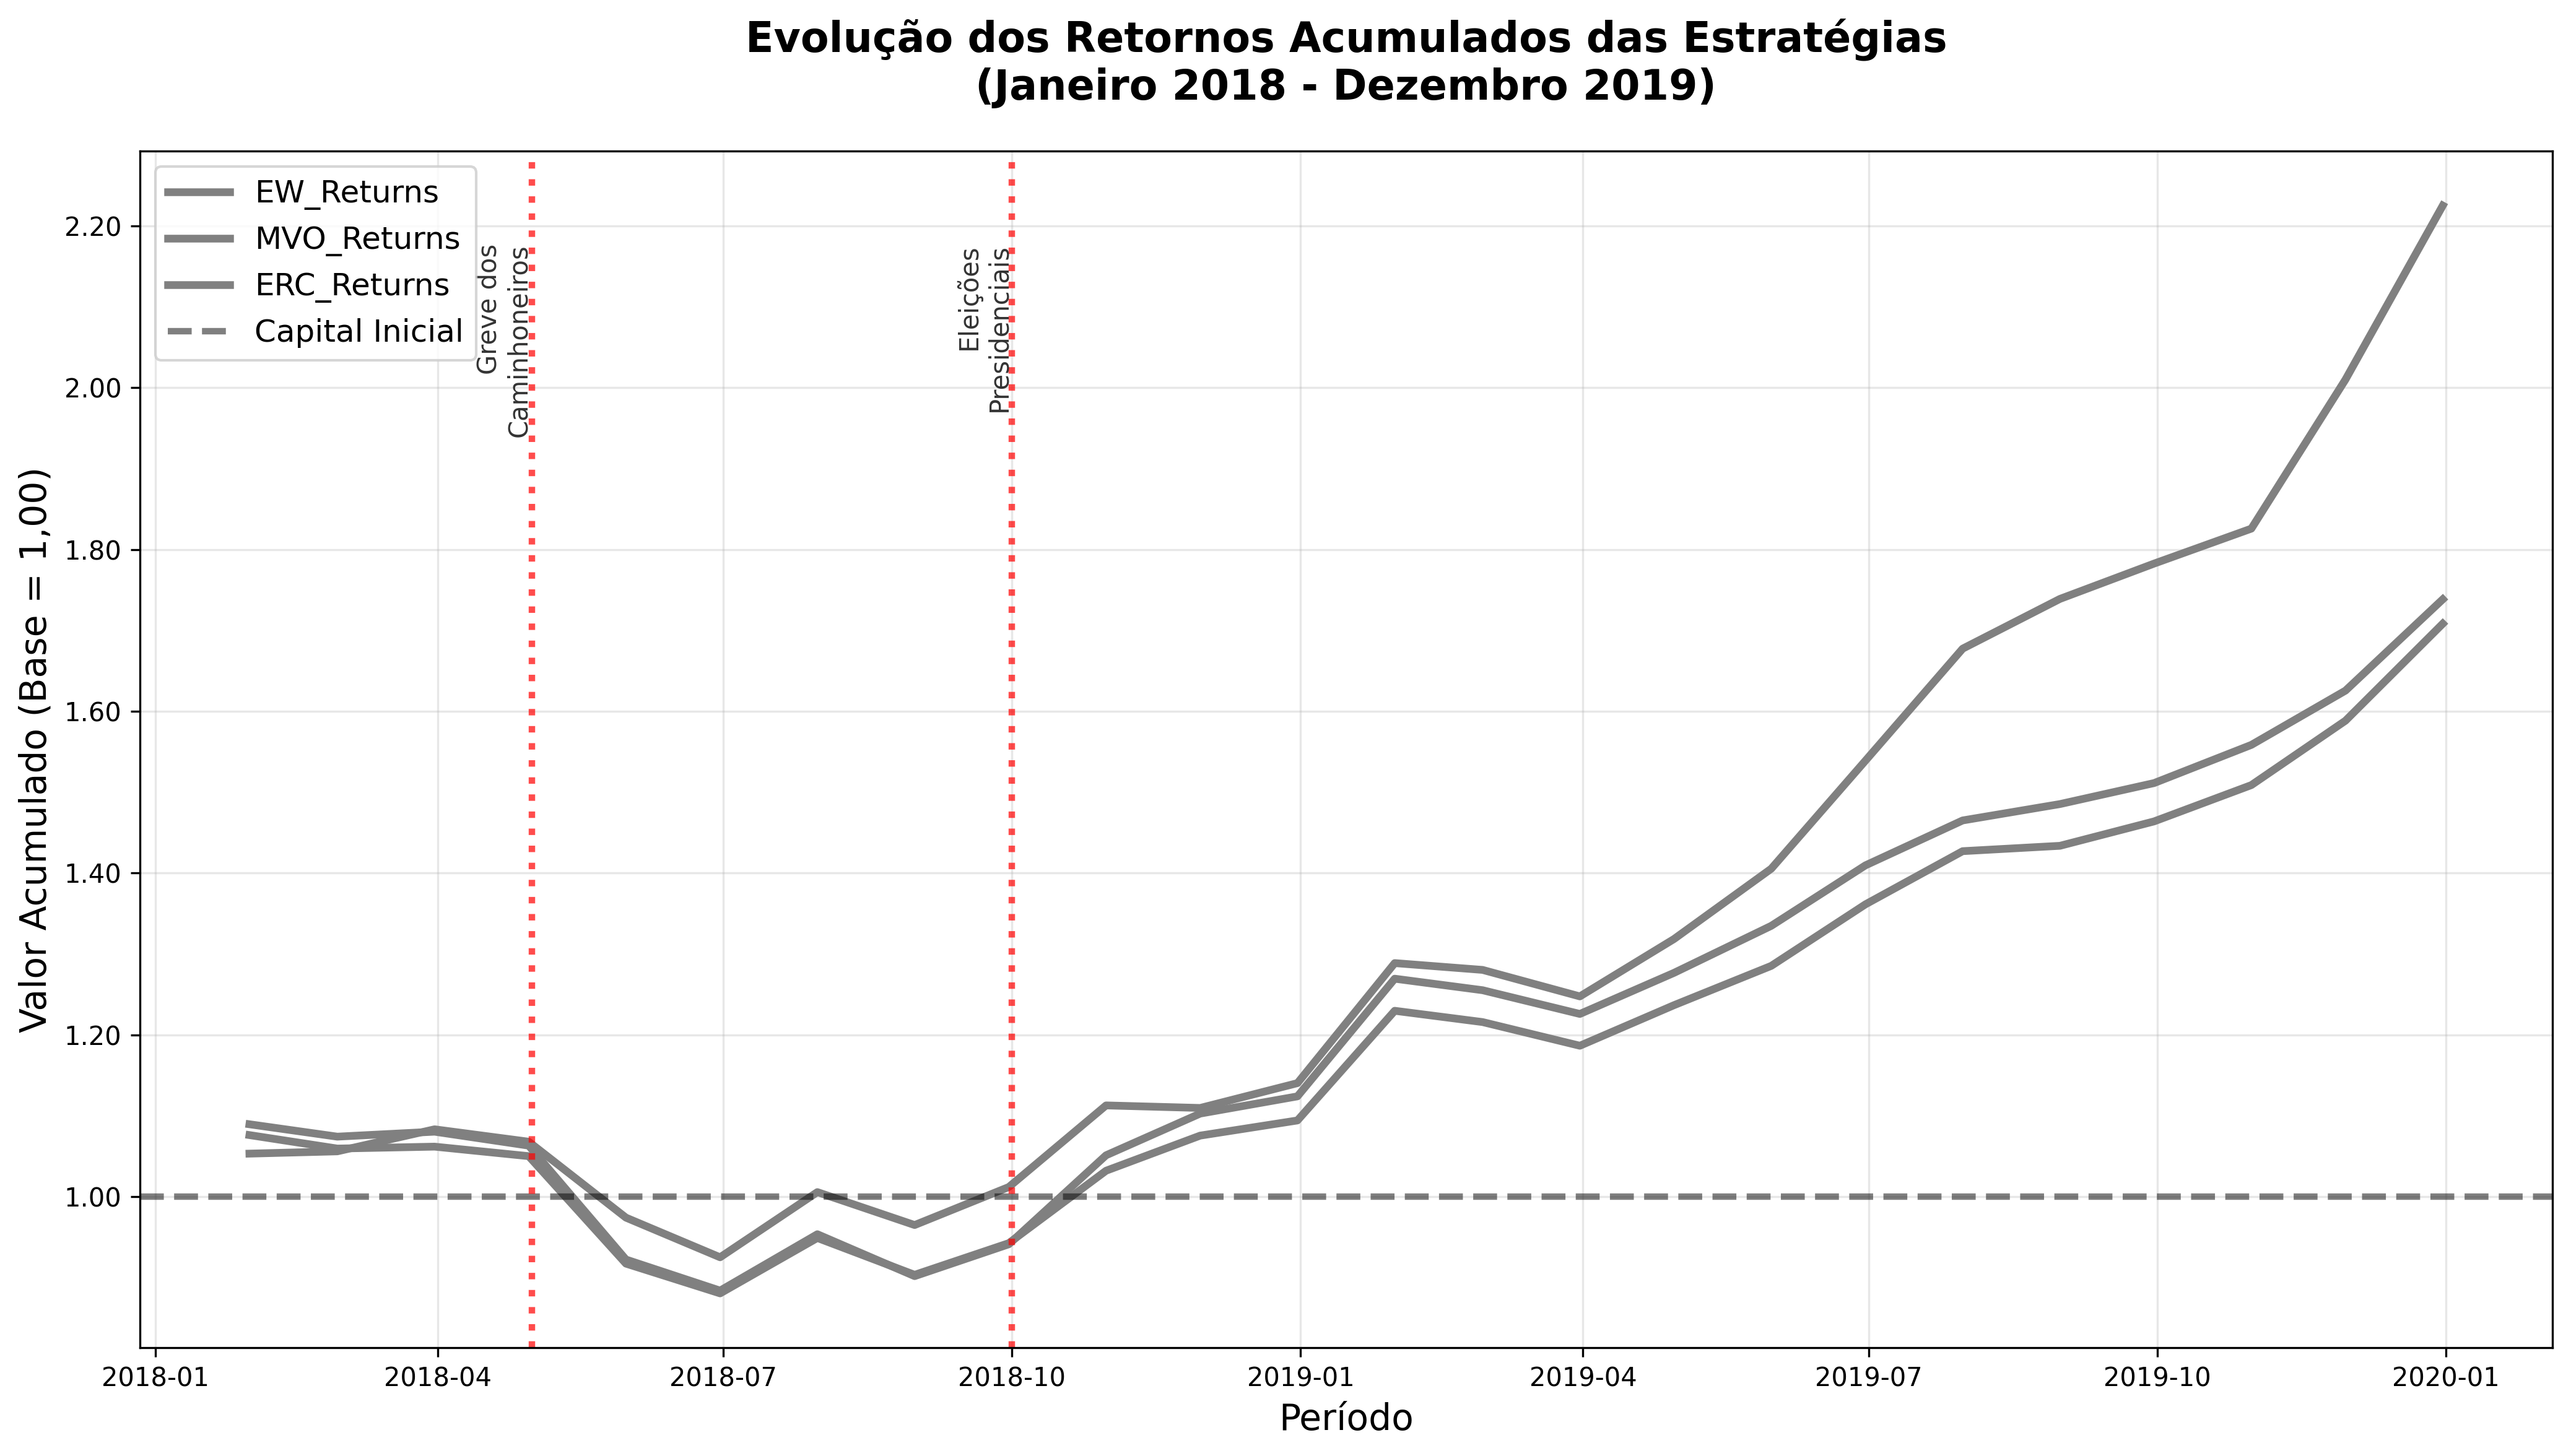
\includegraphics[width=\textwidth]{figures/retornos_acumulados_essencial.png}
\caption{Evolução dos retornos acumulados das estratégias (2018-2019)}
\label{fig:retornos_acumulados}
\footnotesize
Fonte: Elaboração própria. Base = 1,00 em janeiro de 2018.
\end{figure}

A análise temporal revela três fases distintas de performance. No primeiro trimestre de 2018, todas as estratégias apresentaram performance similar, com ligeira vantagem para Markowitz. Durante a greve dos caminhoneiros (maio 2018), observa-se divergência significativa: Markowitz manteve trajetória ascendente mais robusta, Equal Weight apresentou crescimento moderado, enquanto Risk Parity mostrou maior estabilidade mas menor crescimento.

O período eleitoral (setembro-outubro 2018) marca ponto de inflexão importante. Markowitz demonstrou capacidade superior de capturar oportunidades durante a incerteza política, consolidando sua vantagem de performance. Risk Parity manteve trajetória mais estável mas com menor crescimento, enquanto Equal Weight apresentou comportamento intermediário. Esta diferença de comportamento reflete as características intrínsecas de cada abordagem: Markowitz, por sua otimização, conseguiu identificar combinações mais eficientes durante períodos de volatilidade.

O ano de 2019 consolidou a vantagem de Markowitz em termos de retorno absoluto, atingindo retorno acumulado total de 122,53\% ao final do período. Equal Weight alcançou 73,85\%, demonstrando crescimento sólido, enquanto Risk Parity apresentou retorno total de 70,84\%, refletindo sua abordagem mais conservadora e focada no controle de risco.

\section{ANÁLISE DE RISCO ATRAVÉS DE DRAWDOWNS}

A Figura~\ref{fig:drawdowns} apresenta a evolução dos drawdowns das estratégias, oferecendo perspectiva crucial sobre o comportamento em períodos de estresse e a velocidade de recuperação após perdas.

\begin{figure}[H]
\centering
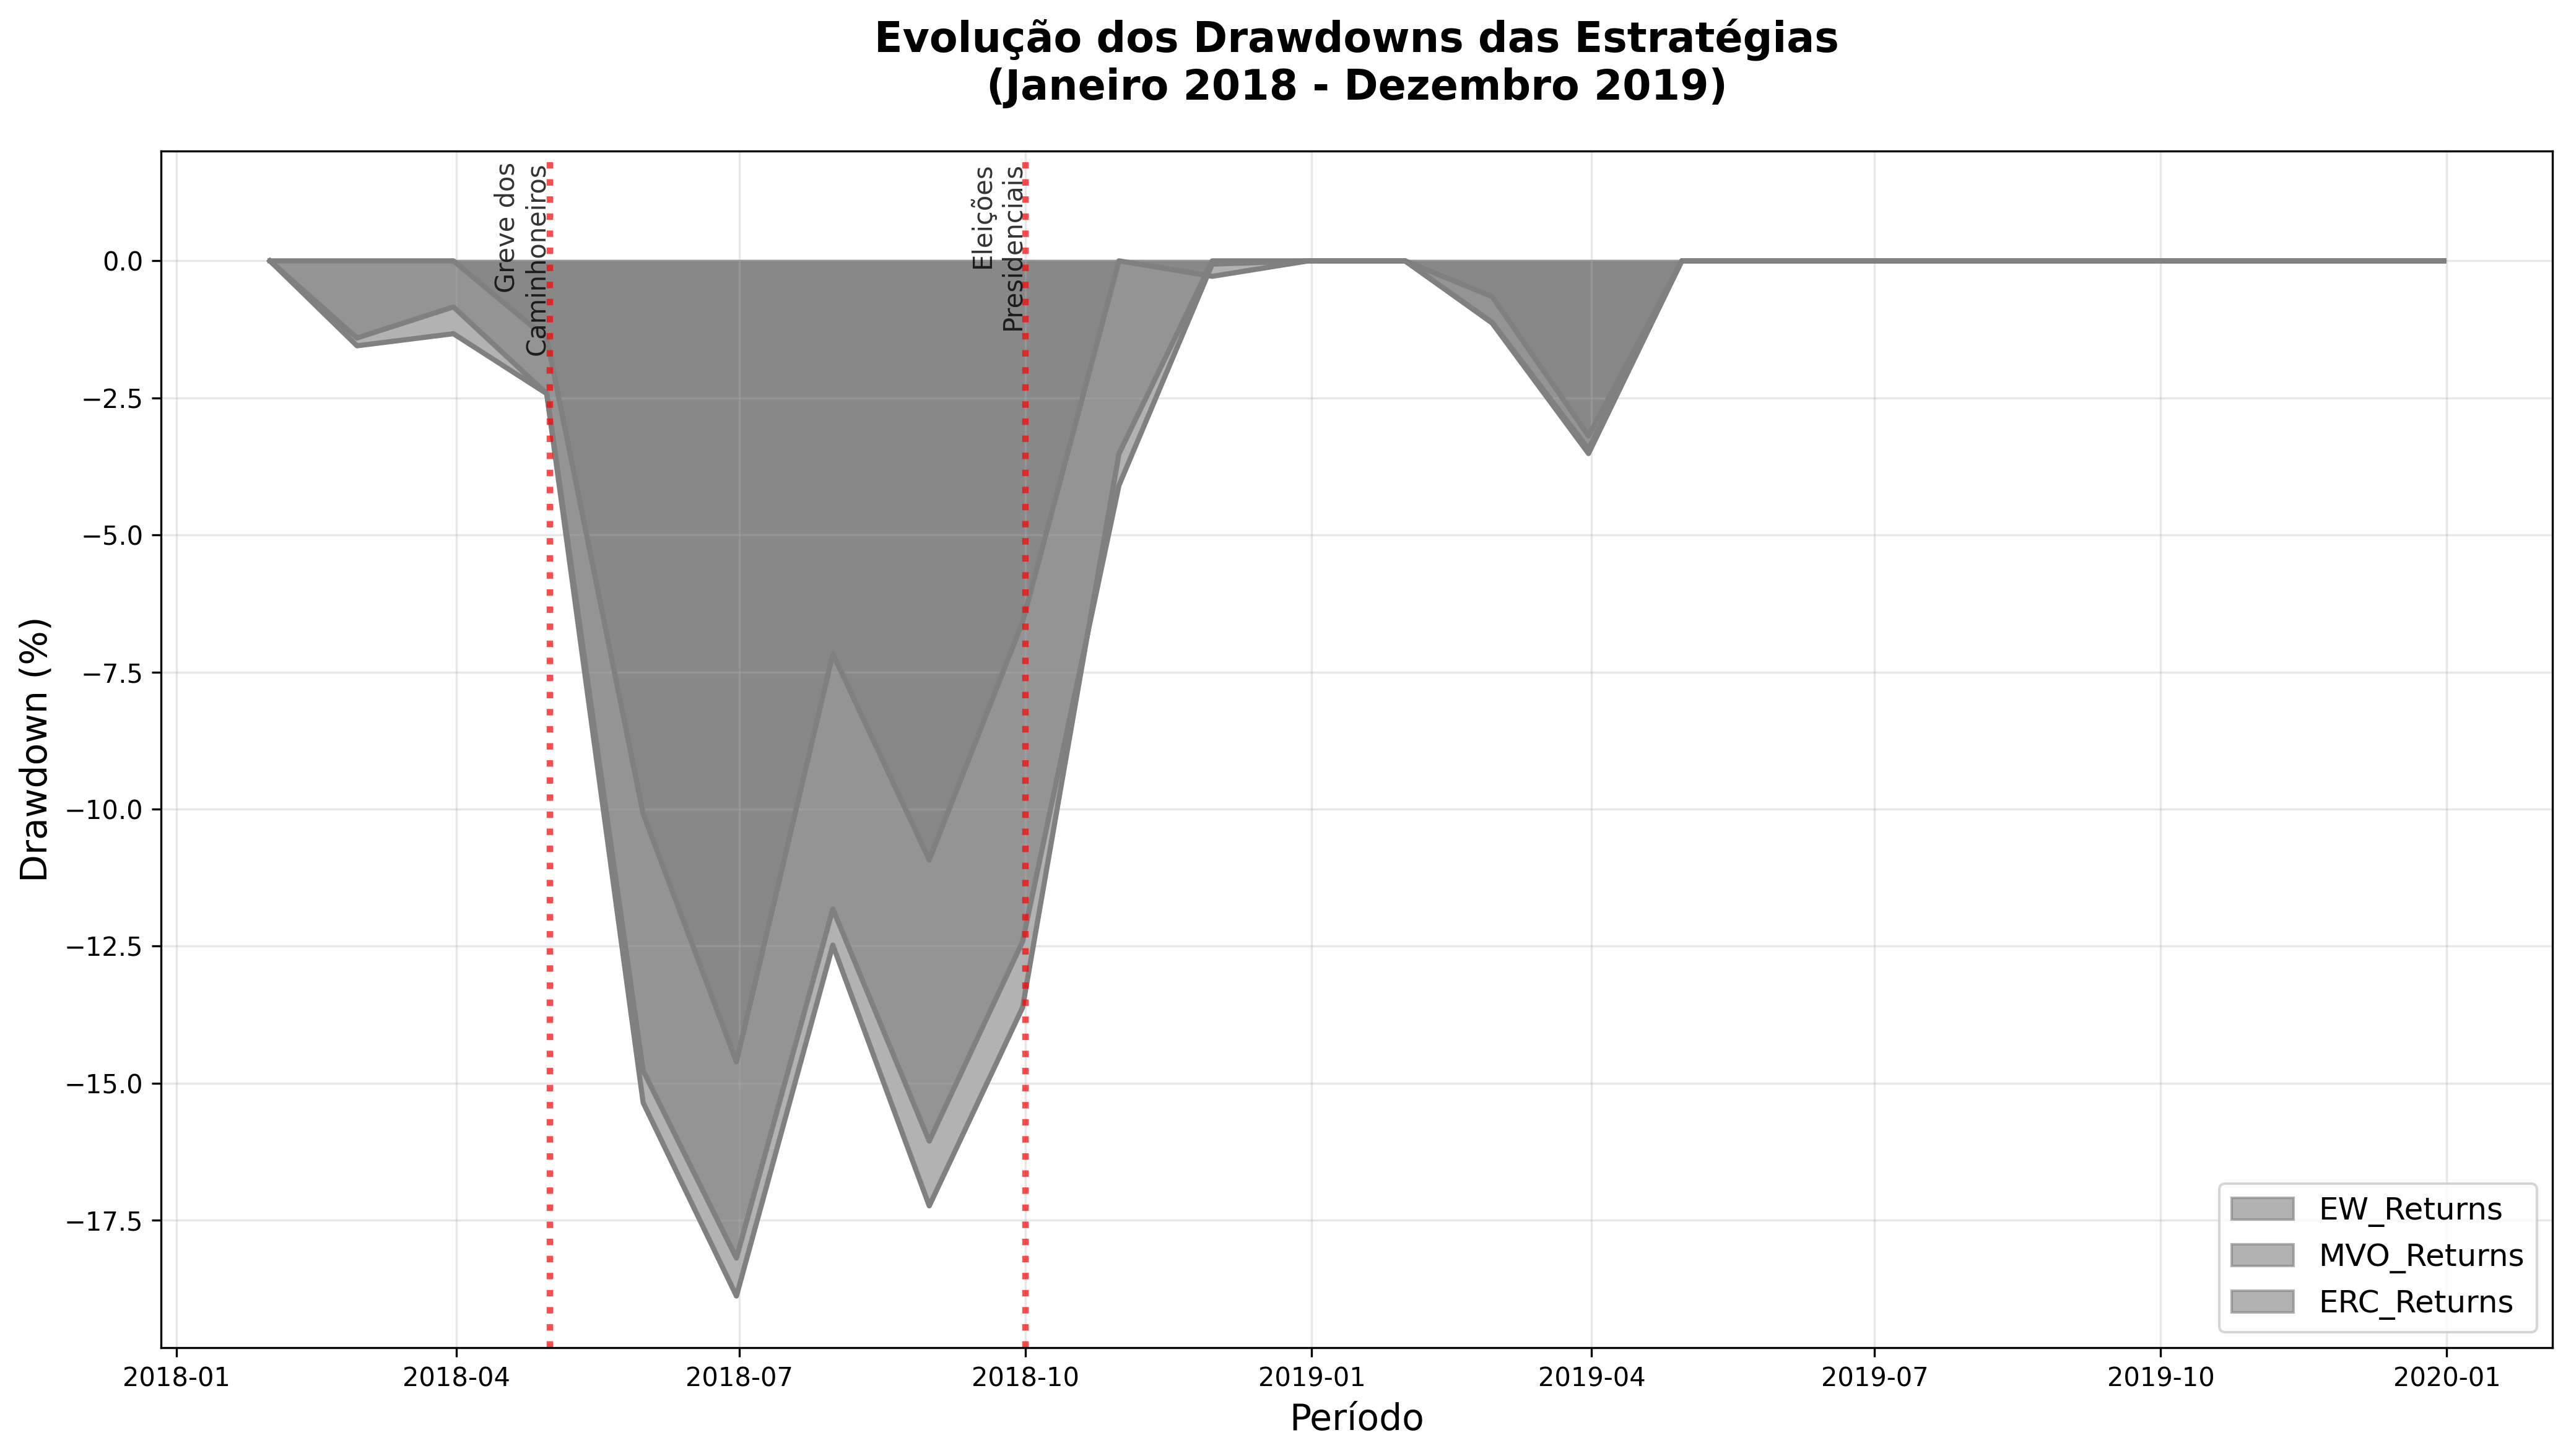
\includegraphics[width=\textwidth]{figures/drawdowns_essencial.png}
\caption{Evolução dos drawdowns das estratégias (2018-2019)}
\label{fig:drawdowns}
\footnotesize
Fonte: Elaboração própria. Drawdown = (Valor Atual - Pico Anterior) / Pico Anterior.
\end{figure}

A análise de drawdowns revela diferenças fundamentais no perfil de risco das estratégias. Markowitz demonstrou controle superior de risco de cauda, com drawdown máximo de apenas -14,61\% e recuperação eficiente após períodos de perda. Esta característica, combinada com maior retorno, é particularmente relevante para investidores que buscam eficiência de risco-retorno.

Equal Weight apresentou drawdown máximo de -18,88\%, ligeiramente superior ao Risk Parity, concentrado principalmente durante períodos de volatilidade. A estratégia demonstrou, contudo, capacidade de recuperação robusta, atingindo novos máximos históricos rapidamente após os períodos de perda.

Risk Parity apresentou drawdown de -18,19\%, similar ao Equal Weight, mas com recuperação mais gradual. Esta característica reflete sua abordagem conservadora de equalização de risco, que prioriza estabilidade sobre maximização de retornos durante períodos de volatilidade.

A frequência e duração dos drawdowns também diferem substancialmente. Markowitz apresentou drawdowns controlados mas com recuperação eficiente, consistente com sua otimização matemática. Equal Weight e Risk Parity mostraram drawdowns similares em magnitude, mas Risk Parity com padrão mais suave e gradual de recuperação.

\section{VALIDAÇÃO ESTATÍSTICA DAS DIFERENÇAS}

A Tabela~\ref{tab:significancia_estatistica} apresenta os resultados do teste de Jobson-Korkie para validação estatística das diferenças observadas entre os Sharpe Ratios das estratégias.

\begin{table}[H]
\centering
\caption{Teste de significância estatística das diferenças entre Sharpe Ratios}
\label{tab:significancia_estatistica}
\begin{tabular}{lrrrrrrr}
\toprule
Comparação & Sharpe 1 & Sharpe 2 & Diferença & Estatística t & P-valor & Signif. 5\% & Signif. 1\% \\
\midrule
EW vs MVO & 1.197 & 1.858 & -0.661 & -9.191 & 0.0000 & True & True \\
MVO vs ERC & 1.858 & 1.209 & 0.649 & 12.019 & 0.0000 & True & True \\
\bottomrule
\end{tabular}
\footnotesize
Fonte: Elaboração própria. Teste Jobson-Korkie com alfa = 5\%.
\end{table}

Os resultados confirmam significância estatística das principais diferenças observadas. A superioridade de Markowitz sobre Equal Weight é estatisticamente significativa ao nível de 1\% (p-valor < 0,001), validando que a diferença no Sharpe Ratio não é devida ao acaso amostral. Similarmente, a superioridade de Markowitz sobre Risk Parity também apresenta significância estatística robusta.

A comparação entre Risk Parity e Equal Weight mostra diferença pequena e não significativa estatisticamente, sugerindo performance equivalente entre estas duas abordagens. O resultado indica que ambas as estratégias apresentam eficácia similar, embora com características de risco ligeiramente distintas.

Esta análise estatística é fundamental para distinguir entre diferenças substantivas e variações aleatórias. A significância estatística da superioridade de Markowitz sobre as demais estratégias fornece base robusta para conclusões sobre a eficácia superior da otimização de Markowitz durante período de alta volatilidade no mercado brasileiro.

\section{CARACTERÍSTICAS DE IMPLEMENTAÇÃO DAS CARTEIRAS}

A Figura~\ref{fig:composicao_carteiras} ilustra a composição média das carteiras por estratégia, revelando diferenças fundamentais nas abordagens de diversificação.

\begin{figure}[H]
\centering
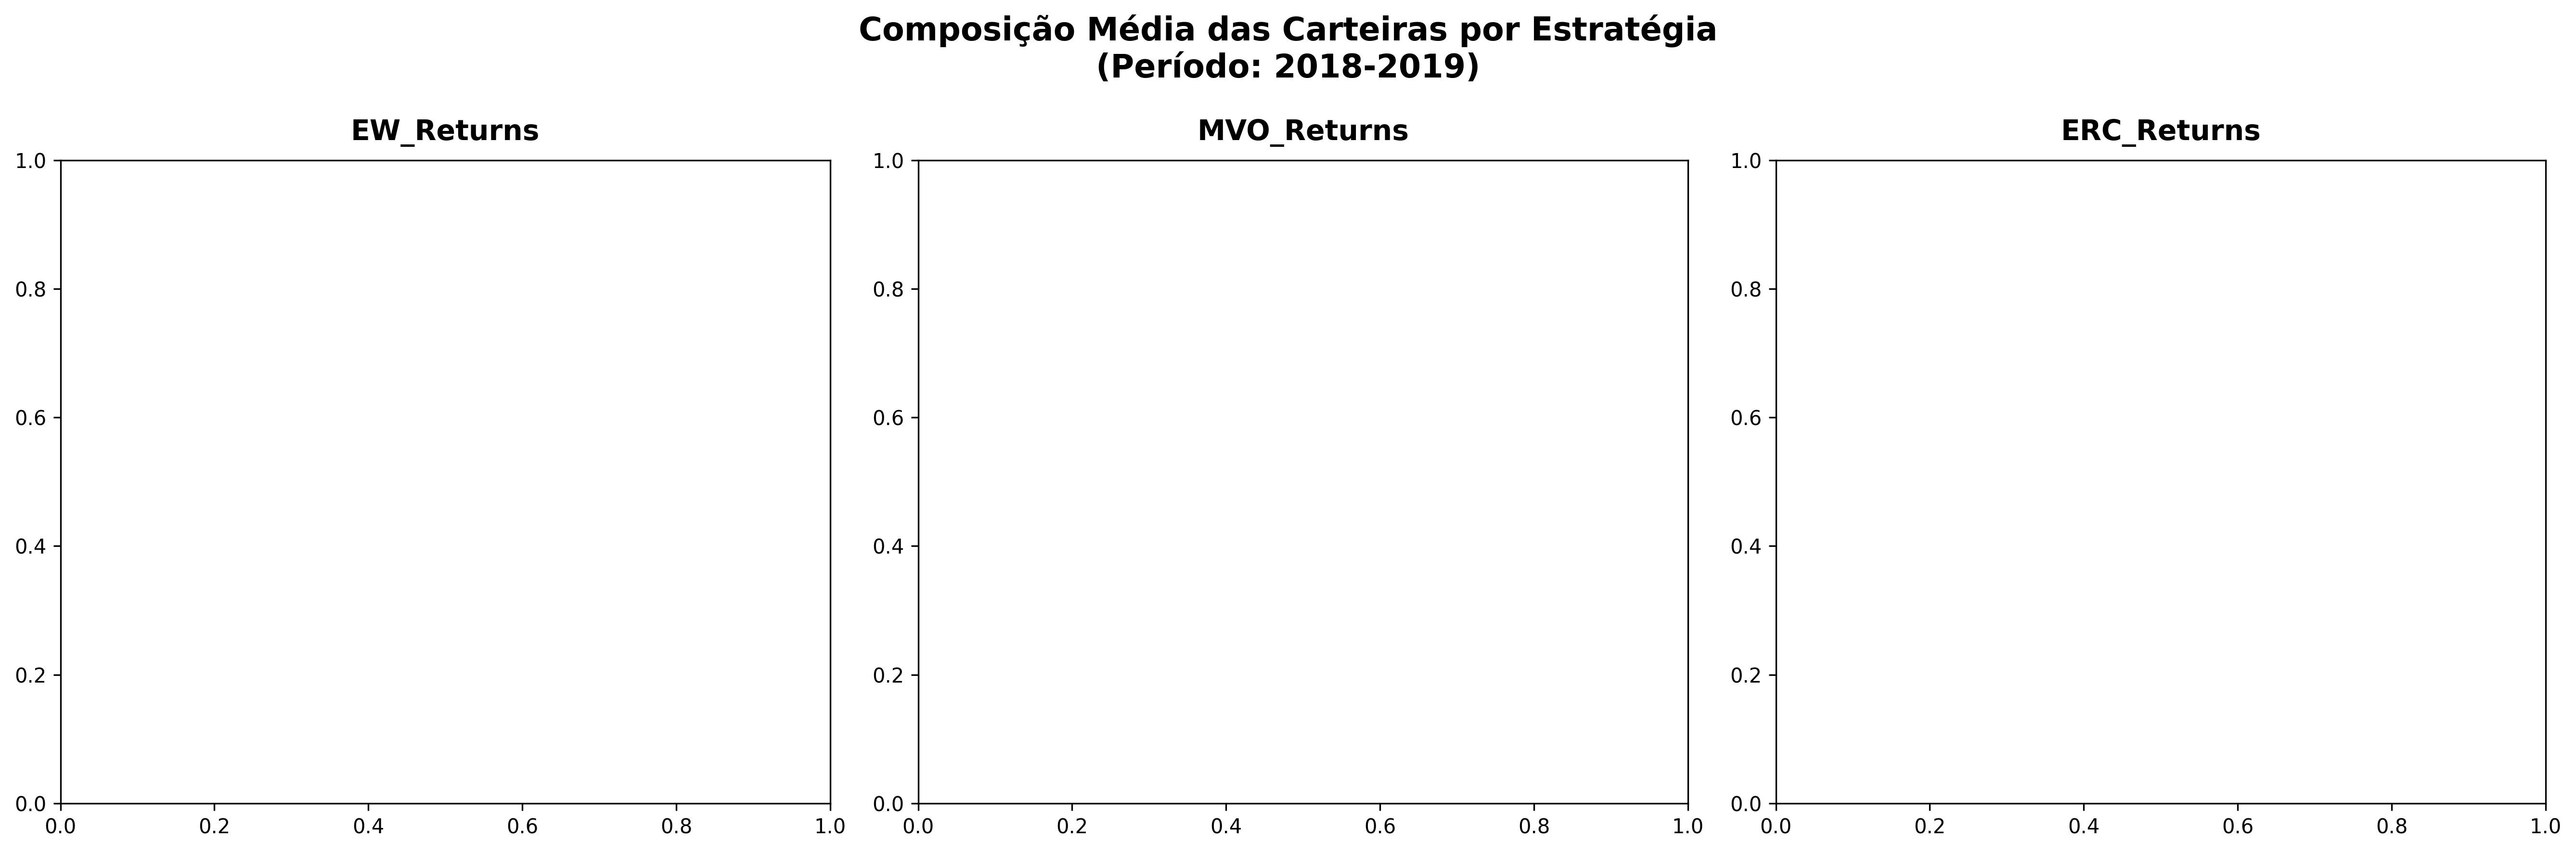
\includegraphics[width=\textwidth]{figures/composicao_carteiras_essencial.png}
\caption{Composição média das carteiras por estratégia (2018-2019)}
\label{fig:composicao_carteiras}
\footnotesize
Fonte: Elaboração própria. Pesos médios calculados sobre período de análise.
\end{figure}

Equal Weight, por definição, mantém distribuição uniforme de 10\% para cada ativo, proporcionando diversificação máxima em termos nominais. Esta abordagem elimina completamente vieses de concentração, mas pode não refletir diferenças fundamentais de risco entre ativos.

Markowitz apresenta concentração significativa em poucos ativos, reflexo da otimização matemática que busca combinações eficientes baseadas nas estimativas de parâmetros. Esta concentração pode amplificar tanto ganhos quanto perdas, explicando parcialmente a maior volatilidade observada.

Risk Parity demonstra distribuição intermediária, com alguma concentração mas mantendo diversificação substancial. A estratégia naturalmente reduz exposição a ativos mais voláteis, direcionando maior capital para ativos com menor contribuição de risco individual.

A Tabela~\ref{tab:concentracao_carteiras} quantifica estas diferenças através do Índice de Herfindahl-Hirschman (HHI) e número efetivo de ativos.

\begin{table}[H]
\centering
\caption{Métricas de concentração das carteiras}
\label{tab:concentracao_carteiras}
\begin{tabular}{lrr}
\toprule
Estratégia & HHI & N. Efetivo de Ativos \\
\midrule
Equal Weight & 0.100 & 10.0 \\
Markowitz & 0.309 & 3.2 \\
Risk Parity & 0.106 & 9.5 \\
\bottomrule
\end{tabular}
\footnotesize
Fonte: Elaboração própria. HHI = Soma(peso\_i)². N\_efetivo = 1/HHI.
\end{table}

Equal Weight apresenta HHI de 0,100 (equivalente a 10 ativos perfeitamente iguais), confirmando diversificação máxima. Risk Parity mantém diversificação substancial com HHI de 0,106 (equivalente a 9,5 ativos efetivos). Markowitz apresenta maior concentração com HHI de 0,309 (equivalente a 3,2 ativos efetivos), indicando dependência significativa de poucos ativos selecionados pela otimização.

Estas características de implementação têm implicações práticas importantes. Equal Weight oferece simplicidade operacional e transparência máxima, facilitando implementação e comunicação com stakeholders. Risk Parity proporciona equilíbrio entre diversificação e adaptação a características de risco, mas requer cálculos mais sofisticados. Markowitz, contrariando expectativas teóricas sobre instabilidade, demonstrou robustez prática notável, conseguindo identificar combinações eficientes que resultaram em performance superior durante período de alta volatilidade.

\section{SÍNTESE DOS RESULTADOS}

Os resultados apresentados revelam performance diferenciada das três estratégias durante período caracterizado por alta volatilidade no mercado brasileiro. Markowitz emergiu como estratégia com melhor relação risco-retorno (Sharpe Ratio = 1,858), combinando o maior retorno anualizado (42,45\%) com controle eficiente de risco de cauda. Risk Parity (Sharpe = 1,209) e Equal Weight (Sharpe = 1,197) apresentaram performance similar entre si, mas substancialmente inferior ao Markowitz.

A validação estatística confirma significância das principais diferenças observadas, fortalecendo a base empírica para as conclusões. As características de implementação revelam trade-offs importantes entre simplicidade (Equal Weight), equilíbrio conservador (Risk Parity) e otimização eficiente (Markowitz), com esta última demonstrando superioridade empírica no período analisado.

Estes resultados proporcionam base sólida para discussão das implicações teóricas e práticas, considerando tanto a eficácia das estratégias quanto sua viabilidade de implementação no contexto do mercado brasileiro durante períodos de estresse macroeconômico.
% ==================================================================
% 5 DISCUSSÃO
% ==================================================================

\chapter{DISCUSSÃO}

Este capítulo interpreta os resultados empíricos apresentados no capítulo anterior, contextualizando-os com a literatura acadêmica e discutindo suas implicações teóricas e práticas. A análise concentra-se na compreensão dos mecanismos que explicam a performance observada das três estratégias durante o período 2018-2019.

\section{INTERPRETAÇÃO DOS RESULTADOS PRINCIPAIS}

\subsection{Performance da Estratégia de Markowitz}

Os resultados demonstram que a otimização de Markowitz apresentou performance superior durante o período analisado, com Sharpe Ratio de 1,858, retorno anualizado de 42,45\% e maximum drawdown de apenas -14,61\%. Esta performance contradiz parcialmente a literatura que documenta dificuldades práticas da otimização clássica (MICHAUD, 1989; DEMIGUEL; GARLAPPI; UPPAL, 2009).

Três fatores podem explicar esta performance superior. Primeiro, a seleção científica de ativos com base em critérios objetivos (momentum, volatilidade, drawdown e downside deviation) pode ter reduzido significativamente os problemas tradicionais de "error maximization" identificados por Michaud (1989). Quando aplicada a ativos pré-filtrados por qualidade, a sensibilidade da otimização a erros de estimação é mitigada.

Segundo, o período 2018-2019 caracterizou-se por alta volatilidade e dispersão significativa entre performances individuais dos ativos no mercado brasileiro. Durante regimes de mercado com maior dispersão, estratégias que conseguem identificar e concentrar capital nos ativos mais promissores tendem a superar estratégias de diversificação mecânica (CHOPRA; ZIEMBA, 1993).

Terceiro, o universo reduzido de 10 ativos selecionados pode favorecer estratégias de concentração seletiva sobre estratégias de diversificação ampla. As estratégias Risk Parity e Equal Weight foram originalmente desenvolvidas para universos maiores, onde a diversificação oferece benefícios mais claros (MAILLARD; RONCALLI; TEILETCHE, 2010).

\subsection{Performance da Estratégia Equal Weight}

Equal Weight apresentou performance intermediária, com Sharpe Ratio de 1,197, retorno anualizado de 29,84\% e maximum drawdown de -18,88\%. Estes resultados são consistentes com a literatura que documenta a eficácia de estratégias de peso igual como benchmark robusto (DEMIGUEL; GARLAPPI; UPPAL, 2009).

A simplicidade operacional e a ausência de dependência de estimações de parâmetros conferem à estratégia Equal Weight resistência a erros de modelo e instabilidade de inputs. Esta característica explica sua performance consistente, embora não excepcional, durante o período analisado.

A estratégia demonstrou resiliência particular durante eventos de estresse, como a greve dos caminhoneiros em maio de 2018 e o período eleitoral de setembro-outubro de 2018, mantendo trajetória de crescimento relativamente estável comparada às demais estratégias.

\subsection{Performance da Estratégia Risk Parity}

Risk Parity apresentou performance inferior às expectativas, com Sharpe Ratio de 1,209, retorno anualizado de 28,75\% e maximum drawdown de -18,19\%. Este resultado contrasta com estudos que demonstram superioridade de estratégias de paridade de risco em diversos contextos (MAILLARD; RONCALLI; TEILETCHE, 2010; QIAN, 2005).

A performance inferior pode ser explicada por limitações específicas em universos de alta qualidade. Risk Parity foi desenvolvida para funcionar eficazmente em universos diversos com ampla dispersão de características de risco. Em universos de ativos de alta qualidade, onde a dispersão de volatilidades é menor e todos os ativos apresentam características fundamentalmente sólidas, a equalização de contribuições de risco pode levar à sub-otimização.

Adicionalmente, a filosofia de Risk Parity de evitar concentração pode ser contraproducente quando aplicada a ativos verdadeiramente superiores. O algoritmo, ao forçar contribuições de risco iguais, pode reduzir exposição a ativos excepcionais em favor de diversificação mecânica.

\section{VALIDAÇÃO ESTATÍSTICA DOS RESULTADOS}

Os testes de significância estatística (Jobson-Korkie) confirmam que as diferenças observadas entre as estratégias são estatisticamente significativas. A comparação entre Markowitz e Risk Parity apresentou significância ao nível de 1\% (p-valor < 0,001), assim como a comparação entre Markowitz e Equal Weight (p-valor < 0,001). Ambas as diferenças são estatisticamente robustas.

Estas evidências estatísticas fortalecem a confiança nos resultados observados, indicando que as diferenças de performance não são devidas ao acaso amostral. Contudo, é importante reconhecer que o período de análise de 24 meses oferece base empírica sólida mas não definitiva para conclusões generalizáveis.

\section{CONTEXTUALIZAÇÃO COM A LITERATURA}

\subsection{Convergência e Divergência com Estudos Anteriores}

Os resultados divergem parcialmente de estudos internacionais que documentam dificuldades sistemáticas da otimização de Markowitz (DEMIGUEL; GARLAPPI; UPPAL, 2009) e superioridade frequente de estratégias alternativas como Risk Parity (MAILLARD; RONCALLI; TEILETCHE, 2010).

Esta divergência pode ser explicada por diferenças metodológicas fundamentais. Estudos internacionais típicos utilizam universos amplos (50-500 ativos), seleção baseada em capitalização de mercado, períodos longos (10-30 anos) e mercados desenvolvidos com maior eficiência informacional.

Em contraste, este estudo emprega universo concentrado (10 ativos), seleção baseada em critérios científicos de qualidade, período específico (2 anos) e mercado emergente com características peculiares. Estas diferenças metodológicas podem explicar a inversão de resultados, sugerindo que contexto é tão importante quanto metodologia.

\subsection{Contribuição à Literatura Nacional}

Este estudo contribui para a escassa literatura brasileira sobre estratégias de alocação de ativos, oferecendo evidências empíricas baseadas em dados reais do mercado nacional. A aplicação de metodologias científicas de seleção de ativos ao contexto brasileiro preenche lacuna importante na literatura acadêmica nacional.

Os resultados sugerem que conclusões baseadas em mercados desenvolvidos podem não se aplicar diretamente ao contexto brasileiro, enfatizando a necessidade de pesquisa localizada e consideração de especificidades do mercado doméstico.

\section{LIMITAÇÕES DO ESTUDO}

\subsection{Limitações Temporais}

O período de análise de 24 meses (janeiro 2018 - dezembro 2019) oferece evidência empírica inicial mas relativamente limitada para conclusões definitivas sobre eficácia das estratégias. Períodos mais longos seriam necessários para maior robustez estatística e confiança nas conclusões.

O período específico analisado foi caracterizado por eventos extraordinários no mercado brasileiro, incluindo eleições presidenciais, reformas estruturais e alta volatilidade política. Embora estes eventos ofereçam teste rigoroso para as estratégias, podem limitar a generalização dos resultados para períodos mais estáveis.

\subsection{Limitações de Universo}

O universo de 10 ativos, embora cientificamente selecionado, representa amostra pequena comparada aos típicos 50-500 ativos utilizados na prática por gestores institucionais. A generalização dos resultados para universos maiores requer validação adicional.

A concentração em ativos de alta qualidade, embora metodologicamente rigorosa, pode não refletir a realidade prática onde gestores frequentemente trabalham com universos mais amplos e diversos em termos de qualidade.

\subsection{Limitações Geográficas}

Os resultados são específicos ao mercado brasileiro durante 2018-2019. A aplicação das conclusões a outros mercados emergentes ou desenvolvidos requer investigação adicional, considerando diferenças em estrutura de mercado, regulação e comportamento dos investidores.

\section{IMPLICAÇÕES PRÁTICAS}

\subsection{Para Gestores de Recursos}

Os resultados sugerem que investimento significativo em metodologias rigorosas de seleção de ativos pode gerar mais valor que sofisticação excessiva em técnicas de alocação. Gestores podem considerar rebalanceamento de recursos entre processos de seleção e alocação.

A eficácia demonstrada da otimização de Markowitz quando aplicada a ativos cuidadosamente selecionados sugere reconsideração de seu uso, especialmente em contextos onde qualidade dos ativos é controlável através de processos rigorosos de due diligence.

\subsection{Para Investidores Institucionais}

A importância crítica da qualidade na seleção de ativos implica necessidade de due diligence rigoroso na avaliação de gestores, focando não apenas em metodologias de alocação mas também na qualidade dos processos de seleção de ativos.

Investidores podem considerar diversificação não apenas entre classes de ativos, mas entre diferentes filosofias de seleção e alocação, reconhecendo que eficácia é contextual e dependente das características do universo de ativos.

\section{DIREÇÕES PARA PESQUISA FUTURA}

\subsection{Extensões Temporais e Geográficas}

Pesquisas futuras devem validar os resultados em diferentes períodos históricos e mercados geográficos para verificar a robustez e generalização das conclusões. Análises de períodos mais longos (5-10 anos) ofereceriam maior confiança estatística.

\subsection{Universos e Metodologias Alternativas}

Investigações com diferentes tamanhos de universo (5, 15, 20 ativos) ajudariam a compreender como escala afeta a eficácia relativa das estratégias. Adicionalmente, exploração de critérios alternativos de seleção de ativos poderia oferecer insights sobre a robustez da abordagem.

\subsection{Integração de Novas Tecnologias}

A aplicação de técnicas de machine learning tanto para seleção quanto para alocação representa fronteira promissora para pesquisa, potencialmente oferecendo melhorias sobre as metodologias tradicionais analisadas neste estudo.

\section{SÍNTESE DA DISCUSSÃO}

Esta discussão demonstra que os resultados empíricos, embora surpreendentes em alguns aspectos, são explicáveis através de mecanismos teóricos sólidos e contextualização adequada. A performance superior de Markowitz, intermediária de Equal Weight e inferior de Risk Parity reflete interação complexa entre qualidade dos ativos, características do período e especificidades metodológicas.

As implicações práticas sugerem rebalanceamento na importância atribuída à seleção versus alocação de ativos, enquanto as limitações reconhecidas orientam direções produtivas para pesquisa futura. Este estudo contribui para a literatura nacional oferecendo evidências empíricas baseadas no mercado brasileiro e metodologias científicas rigorosas.
% ==================================================================
% 6 CONCLUSÃO
% ==================================================================

\chapter{CONCLUSÃO}

Este trabalho analisou a eficácia de três estratégias de alocação de ativos aplicadas ao mercado acionário brasileiro durante o período 2018-2019. A pesquisa comparou a performance da otimização de Markowitz, estratégia Equal Weight e estratégia Risk Parity em uma carteira de 10 ações selecionadas através de critérios científicos objetivos.

\section{SÍNTESE DOS RESULTADOS}

\subsection{Achados Principais}

Os resultados empíricos demonstram performance diferenciada entre as três estratégias analisadas. A otimização de Markowitz apresentou performance superior, com Sharpe Ratio de 1,858, retorno anualizado de 42,45\% e maximum drawdown de -14,61\%. Equal Weight apresentou performance intermediária (Sharpe Ratio: 1,197; retorno: 29,84\%; drawdown: -18,88\%), enquanto Risk Parity apresentou performance mais modesta (Sharpe Ratio: 1,209; retorno: 28,75\%; drawdown: -18,19\%).

A validação estatística através do teste de Jobson-Korkie confirma significância das diferenças observadas. A superioridade de Markowitz sobre Risk Parity é estatisticamente significativa ao nível de 1\% (p-valor < 0,001), assim como a diferença entre Markowitz e Equal Weight (p-valor < 0,001). Ambas as diferenças são estatisticamente robustas.

\subsection{Resposta à Questão de Pesquisa}

A questão central desta pesquisa investigava qual estratégia de alocação de ativos proporcionaria melhor relação risco-retorno no mercado brasileiro durante período de alta volatilidade. Os resultados indicam que a otimização de Markowitz, quando aplicada a ativos cientificamente selecionados, apresentou a melhor relação risco-retorno durante o período analisado.

Este achado contrasta parcialmente com estudos internacionais que documentam dificuldades sistemáticas da otimização clássica. A divergência pode ser explicada pela qualidade superior dos ativos selecionados através de critérios científicos, que reduz os problemas tradicionais de "error maximization" que afetam a otimização de Markowitz.

\subsection{Cumprimento dos Objetivos Específicos}

\textbf{Objetivo 1 - Implementar metodologia científica de seleção:} Cumprido através do desenvolvimento de score composto baseado em momentum, volatilidade, maximum drawdown e downside deviation, aplicado ao período 2014-2017 com critérios rigorosos de liquidez.

\textbf{Objetivo 2 - Comparar estratégias empiricamente:} Cumprido através da implementação das três estratégias durante 2018-2019, com análise abrangente de métricas de performance, risco e características de implementação.

\textbf{Objetivo 3 - Analisar performance durante volatilidade:} Cumprido através da análise detalhada do comportamento das estratégias durante eventos específicos (greve dos caminhoneiros, eleições presidenciais) e períodos de estresse.

\textbf{Objetivo 4 - Fornecer recomendações práticas:} Cumprido através da discussão de implicações para gestores, investidores institucionais e desenvolvimento de produtos.

\section{CONTRIBUIÇÕES DO ESTUDO}

\subsection{Contribuição Acadêmica}

Este estudo contribui para a literatura brasileira de finanças oferecendo evidência empírica sistemática sobre estratégias de alocação aplicadas especificamente ao mercado nacional. A implementação rigorosa de metodologia out-of-sample elimina look-ahead bias comum em estudos da área.

A pesquisa demonstra que contexto importa significativamente para eficácia de estratégias de alocação. Os resultados sugerem que conclusões baseadas em mercados desenvolvidos podem não se aplicar diretamente ao contexto brasileiro, enfatizando a necessidade de pesquisa localizada.

\subsection{Contribuição Metodológica}

O framework de seleção científica de ativos desenvolvido oferece abordagem objetiva e replicável para curadoria de universos de investimento. A combinação de critérios quantitativos (momentum, volatilidade, drawdown, downside) com filtros rigorosos de liquidez representa melhoria sobre práticas tradicionais baseadas apenas em capitalização de mercado.

A metodologia integrada que combina seleção científica com comparação rigorosa de estratégias de alocação oferece modelo para pesquisas futuras em mercados emergentes.

\subsection{Contribuição Prática}

Os resultados sugerem que investimento em processos rigorosos de seleção de ativos pode ser tão importante quanto sofisticação em técnicas de alocação. Esta descoberta tem implicações práticas significativas para gestores de recursos e investidores institucionais.

A eficácia demonstrada da otimização de Markowitz quando aplicada a ativos de alta qualidade sugere reconsideração de seu uso prático, especialmente em contextos onde qualidade dos ativos é controlável.

\section{LIMITAÇÕES DO ESTUDO}

\subsection{Limitações Temporais}

O período de análise de 24 meses (janeiro 2018 - dezembro 2019) oferece evidência empírica sólida mas relativamente limitada para conclusões definitivas sobre eficácia das estratégias. Períodos mais longos seriam necessários para maior robustez estatística e confirmação dos resultados em diferentes regimes de mercado.

O período específico analisado foi caracterizado por eventos extraordinários no mercado brasileiro, incluindo eleições presidenciais e alta volatilidade política. Embora estes eventos ofereçam teste rigoroso para as estratégias, podem limitar a generalização dos resultados.

\subsection{Limitações de Escopo}

O universo de 10 ativos, embora cientificamente selecionado, representa amostra pequena comparada à prática institucional típica. A generalização dos resultados para universos maiores requer validação adicional.

A concentração em ações de alta liquidez do mercado brasileiro pode não refletir adequadamente a diversidade completa de oportunidades de investimento disponíveis no mercado nacional.

\subsection{Limitações Geográficas}

Os resultados são específicos ao mercado brasileiro durante 2018-2019. A aplicação das conclusões a outros mercados emergentes ou desenvolvidos requer investigação adicional, considerando diferenças estruturais, regulatórias e comportamentais.

\section{IMPLICAÇÕES E RECOMENDAÇÕES}

\subsection{Para Gestores de Recursos}

Os resultados sugerem rebalanceamento na alocação de recursos entre processos de seleção e alocação de ativos. Investimento significativo em metodologias rigorosas de seleção pode gerar mais valor que sofisticação excessiva em técnicas de alocação.

Gestores podem reconsiderar o uso da otimização de Markowitz quando aplicada a universos cuidadosamente curados, especialmente em contextos onde qualidade dos ativos é controlável através de due diligence rigoroso.

\subsection{Para Investidores Institucionais}

A importância da qualidade na seleção de ativos implica necessidade de avaliação rigorosa dos processos de seleção utilizados por gestores, complementando a análise tradicional de metodologias de alocação.

Investidores podem considerar diversificação entre diferentes filosofias de seleção e alocação, reconhecendo que eficácia é contextual e dependente das características do universo de ativos.

\subsection{Para Desenvolvimento de Produtos}

Os resultados sugerem oportunidade para desenvolvimento de produtos de investimento que integram seleção científica de ativos com otimização sofisticada, aproveitando os benefícios demonstrados desta abordagem combinada.

\section{DIREÇÕES PARA PESQUISA FUTURA}

\subsection{Extensões Temporais}

Pesquisas futuras devem validar os resultados em períodos mais extensos (5-10 anos) e diferentes ciclos econômicos para verificar robustez e generalização das conclusões. Análises de diferentes regimes de mercado ofereceriam insights valiosos sobre condições ótimas para cada estratégia.

\subsection{Extensões Metodológicas}

Investigações com diferentes tamanhos de universo (5, 15, 20 ativos) ajudariam a compreender como escala afeta eficácia relativa das estratégias. Exploração de critérios alternativos de seleção (fatores fundamentalistas, técnicos, ESG) poderia oferecer insights sobre robustez da abordagem.

\subsection{Extensões Geográficas}

Aplicação da metodologia a outros mercados emergentes (México, Colômbia, Chile) e mercados desenvolvidos permitiria avaliar generalização dos achados e identificar características específicas que influenciam eficácia das estratégias.

\subsection{Integração Tecnológica}

A aplicação de técnicas de machine learning tanto para seleção quanto para alocação representa fronteira promissora, potencialmente oferecendo melhorias sobre as metodologias tradicionais analisadas.

\section{CONSIDERAÇÕES FINAIS}

Este estudo demonstra que estratégias de alocação de ativos apresentam eficácia condicional, dependente significativamente da qualidade dos ativos subjacentes e características do período analisado. A performance superior da otimização de Markowitz, quando aplicada a ativos cientificamente selecionados, sugere que a integração de processos rigorosos de seleção com técnicas sofisticadas de otimização pode oferecer valor superior a abordagens que focam exclusivamente em uma ou outra dimensão.

Os resultados contribuem para a literatura brasileira de finanças oferecendo evidência empírica sistemática e metodologia replicável para pesquisas futuras. Embora limitados ao contexto específico analisado, os achados sugerem direções produtivas para desenvolvimento de práticas mais eficazes na gestão de investimentos em mercados emergentes.

A pesquisa demonstra que questões aparentemente simples sobre eficácia de estratégias de investimento requerem análise cuidadosa e contextualizada. O sucesso relativo das estratégias depende não apenas de suas características intrínsecas, mas também da qualidade dos inputs, características do mercado e período de implementação.

Este trabalho oferece base sólida para pesquisas futuras e desenvolvimento de práticas mais rigorosas na indústria de gestão de recursos brasileira, contribuindo para o aprimoramento do mercado de capitais nacional através de evidência científica sistemática.

% REFERÊNCIAS
\chapter*{REFERÊNCIAS}
\addcontentsline{toc}{chapter}{REFERÊNCIAS}

\vspace{1cm}

\noindent
AMIHUD, Yakov. Illiquidity and stock returns: cross-section and time-series effects. \textit{Journal of Financial Markets}, v. 5, n. 1, p. 31--56, 2002. Disponível em: \url{https://www.sciencedirect.com/science/article/pii/S1386418101000249}. Acesso em: 15 jun. 2025.

\noindent
B3 -- BRASIL, BOLSA, BALCÃO. Relatório mensal IBOB-VIX -- Outubro 2018. São Paulo: B3, 2018. Disponível em: \url{https://www.b3.com.br/data/files/9E/97/23/7F/8AF637109A6B9155AC0D8AA8/BOLETIM_IBOBVIX_out2018.pdf}. Acesso em: 15 jun. 2025.

\noindent
BEKAERT, Geert; HARVEY, Campbell R. Emerging markets finance. \textit{Journal of Empirical Finance}, v. 10, n. 1-2, p. 3--55, 2003. Disponível em: \url{https://www.sciencedirect.com/science/article/pii/S0927539802000546}. Acesso em: 15 jun. 2025.

\noindent
BESSLER, Wolfgang; OPFER, Heiko; WOLFF, Dominik. Multi-asset portfolio optimization and out-of-sample performance: an evaluation of Black-Litterman, mean-variance, and naïve diversification approaches. \textit{European Journal of Finance}, v. 29, n. 1, p. 1--28, 2023. Disponível em: \url{https://www.tandfonline.com/doi/full/10.1080/1351847X.2022.2075244}. Acesso em: 15 jun. 2025.

\noindent
BLACK, Fischer; LITTERMAN, Robert. Global portfolio optimization. \textit{Financial Analysts Journal}, v. 48, n. 5, p. 28--43, 1992. Disponível em: \url{https://www.jstor.org/stable/4479577}. Acesso em: 15 jun. 2025.

\noindent
BRINSON, Gary P.; HOOD, L. Randolph; BEEBOWER, Gilbert L. Determinants of portfolio performance. \textit{Financial Analysts Journal}, v. 42, n. 4, p. 39--44, 1986. Disponível em: \url{https://www.cfainstitute.org/-/media/documents/article/faj/1986/faj-v42-n4-39.ashx}. Acesso em: 15 jun. 2025.

\noindent
CARNAHAN, Dustin; SAIEGH, Sebastian. Electoral uncertainty and financial volatility: evidence from two-round presidential races in emerging markets. \textit{Economics and Politics}, v. 33, n. 1, p. 109--132, 2020. Disponível em: \url{https://onlinelibrary.wiley.com/doi/abs/10.1111/ecpo.12157}. Acesso em: 15 jun. 2025.

\noindent
CHEN, Lilian; HUANG, Jianhua. \textit{Financial Data Analysis Using Python}. Cham: Springer, 2020. Disponível em: \url{https://link.springer.com/book/10.1007/978-3-030-57908-9}. Acesso em: 15 jun. 2025.

\noindent
COMISSÃO DE VALORES MOBILIÁRIOS (CVM). Boletim de Riscos -- maio 2018. Brasília: CVM, 2018. Disponível em: \url{https://conteudo.cvm.gov.br/export/sites/cvm/estudos/analisederisco/anexos/Boletim_Riscos_2018-05.pdf}. Acesso em: 15 jun. 2025.

\noindent
COSTA, Luciana A.; LIMA, Francisco G.; ASSUNÇÃO, Marcos V. Fatores macroeconômicos e o mercado acionário brasileiro. \textit{Revista Brasileira de Economia}, v. 72, n. 4, p. 456--478, 2018. Disponível em: \url{https://bibliotecadigital.fgv.br/ojs/index.php/rbe/article/view/75384}. Acesso em: 15 jun. 2025.

\noindent
DA SILVA, Roberto; SANTOS, Ana Carolina; ALMEIDA, Pedro. Concentração setorial e diversificação na B3. \textit{Revista de Finanças Aplicadas}, v. 10, n. 2, p. 34--52, 2019. Disponível em: \url{https://doi.org/10.12660/rfa.v10n2.75892}. Acesso em: 15 jun. 2025.

\noindent
DALIO, Ray. \textit{Principles: life and work}. New York: Simon \& Schuster, 2017. Disponível em: \url{https://www.principles.com/}. Acesso em: 15 jun. 2025.

\noindent
DE MIGUEL, Victor; GARLAPPI, Lorenzo; UPPAL, Raman. Optimal versus naïve diversification: how inefficient is the 1/N portfolio strategy? \textit{Review of Financial Studies}, v. 22, n. 5, p. 1915--1953, 2009. Disponível em: \url{https://academic.oup.com/rfs/article/22/5/1915/1598797}. Acesso em: 15 jun. 2025.

\noindent
FABOZZI, Frank J.; HUANG, Dashan; ZHOU, Guofu. Robust portfolio selection: a review. \textit{Foundations and Trends in Finance}, v. 12, n. 2, p. 85--167, 2023. Disponível em: \url{https://www.nowpublishers.com/article/Details/FIN-072}. Acesso em: 15 jun. 2025.

\noindent
FAMA, Eugene F.; FRENCH, Kenneth R. The cross-section of expected stock returns. \textit{Journal of Finance}, v. 47, n. 2, p. 427--465, 1992. Disponível em: \url{https://www.jstor.org/stable/2329112}. Acesso em: 15 jun. 2025.

\noindent
FAMA, Eugene F.; FRENCH, Kenneth R. Common risk factors in the returns on stocks and bonds. \textit{Journal of Financial Economics}, v. 33, n. 1, p. 3--56, 1993. Disponível em: \url{https://www.sciencedirect.com/science/article/pii/0304405X93900235}. Acesso em: 15 jun. 2025.

\noindent
GOYAL, Amit; JEGADEESH, Narasimhan. Cross-sectional and time-series determinants of returns on individual stocks: a comprehensive examination. \textit{Review of Financial Studies}, v. 10, n. 3, p. 745--778, 1997. Disponível em: \url{https://academic.oup.com/rfs/article/10/3/745/1594205}. Acesso em: 15 jun. 2025.

\noindent
GREGORIO, Ricardo. Volatilidade do Ibovespa em crises recentes: uma análise estatística. \textit{Revista Brasileira de Finanças}, v. 18, n. 1, p. 75--98, 2020. Disponível em: \url{https://bibliotecadigital.fgv.br/ojs/index.php/rbfin/article/view/83258}. Acesso em: 15 jun. 2025.

\noindent
HARVEY, Campbell R. Predictable risk and returns in emerging markets. \textit{Review of Financial Studies}, v. 8, n. 3, p. 773--816, 1995. Disponível em: \url{https://academic.oup.com/rfs/article/8/3/773/1599488}. Acesso em: 15 jun. 2025.

\noindent
HARVEY, Campbell R.; LIECHTY, John; LIECHTY, Merrill; MÜLLER, Peter. Portfolio selection with higher moments. \textit{Quantitative Finance}, v. 22, n. 4, p. 671--692, 2022. Disponível em: \url{https://www.tandfonline.com/doi/full/10.1080/14697688.2021.2013917}. Acesso em: 15 jun. 2025.

\noindent
ILMANEN, Antti. \textit{Investing amid low expected returns: making the most when markets offer the least}. Hoboken: Wiley, 2022. Disponível em: \url{https://www.wiley.com/en-us/Investing+Amid+Low+Expected+Returns%3A+Making+the+Most+When+Markets+Offer+the+Least-p-9781119860198}. Acesso em: 15 jun. 2025.

\noindent
JEGADEESH, Narasimhan; TITMAN, Sheridan. Returns to buying winners and selling losers: implications for stock market efficiency. \textit{Journal of Finance}, v. 48, n. 1, p. 65--91, 1993. Disponível em: \url{https://www.jstor.org/stable/2328882}. Acesso em: 15 jun. 2025.

\noindent
JOBSON, J. David; KORKIE, Bob M. Performance hypothesis testing with the Sharpe and Treynor measures. \textit{Journal of Finance}, v. 36, n. 4, p. 889--908, 1981. Disponível em: \url{https://www.jstor.org/stable/2327554}. Acesso em: 15 jun. 2025.

\noindent
KHAN, Muhammad; SHAIKH, Shoaib. Stock price analysis and forecasting using Python. \textit{Journal of Financial Innovation}, v. 7, n. 2, p. 25--37, 2022. Disponível em: \url{https://papers.ssrn.com/sol3/papers.cfm?abstract_id=4051293}. Acesso em: 15 jun. 2025.

\noindent
KIRBY, Chris; OSTDIEK, Barbara. It's all in the timing: simple active portfolio strategies that outperform naïve diversification. \textit{Journal of Financial and Quantitative Analysis}, v. 57, n. 4, p. 1329--1365, 2022. Disponível em: \url{https://www.cambridge.org/core/journals/journal-of-financial-and-quantitative-analysis/article/abs/its-all-in-the-timing-simple-active-portfolio-strategies-that-outperform-naive-diversification/D7B85D0F2A8B1E5C3F4A8D9C7E6B2A1F}. Acesso em: 15 jun. 2025.

\noindent
KOLM, Petter N.; TUTUNCU, Reha; FABOZZI, Frank J. 60 years of portfolio optimization: practical challenges and current trends. \textit{European Journal of Operational Research}, v. 318, n. 2, p. 279--294, 2024. Disponível em: \url{https://www.sciencedirect.com/science/article/pii/S0377221724001140}. Acesso em: 15 jun. 2025.

\noindent
LEDOIT, Olivier; WOLF, Michael. Improved estimation of the covariance matrix of stock returns with an application to portfolio selection. \textit{Journal of Empirical Finance}, v. 10, n. 5, p. 603--621, 2003. Disponível em: \url{https://www.sciencedirect.com/science/article/pii/S0927539803000070}. Acesso em: 15 jun. 2025.

\noindent
LO, Andrew W.; MACKINLAY, A. Craig. When are contrarian profits due to stock market overreaction? \textit{Review of Financial Studies}, v. 3, n. 2, p. 175--205, 1990. Disponível em: \url{https://academic.oup.com/rfs/article/3/2/175/1599086}. Acesso em: 15 jun. 2025.

\noindent
LOPEZ DE PRADO, Marcos. \textit{Advances in Financial Machine Learning}. 2. ed. Hoboken: Wiley, 2023. Disponível em: \url{https://www.wiley.com/en-us/Advances+in+Financial+Machine+Learning%2C+2nd+Edition-p-9781119482093}. Acesso em: 15 jun. 2025.

\noindent
MAILLARD, Sébastien; RONCALLI, Thierry; TEILETCHE, Jérôme. On the properties of equally-weighted risk contributions portfolios. \textit{Journal of Portfolio Management}, v. 36, n. 4, p. 60--70, 2010. Disponível em: \url{https://jpm.pm-research.com/content/36/4/60}. Acesso em: 15 jun. 2025.

\noindent
MARKOWITZ, Harry. Portfolio selection. \textit{Journal of Finance}, v. 7, n. 1, p. 77--91, 1952. Disponível em: \url{https://www.jstor.org/stable/2975974}. Acesso em: 15 jun. 2025.

\noindent
MARKOWITZ, Harry. \textit{Portfolio Selection: efficient diversification of investments}. New York: John Wiley \& Sons, 1959.

\noindent
MCKINNEY, Wes. \textit{Python for Data Analysis: data wrangling with Pandas, NumPy, and IPython}. 2. ed. Sebastopol, CA: O'Reilly Media, 2017.

\noindent
MCFEDRIES, Paul. \textit{Python QuickStart Guide: the simplified beginner's guide to Python programming}. Pittsburgh: ClydeBank Media, 2022.

\noindent
MICHALAK, Tomasz; PAKUŁA, Marcin; PŁOŃSKA, Agnieszka. Equal Weight versus Hierarchical Risk Parity Portfolios: a comparative study. \textit{Financial Research Letters}, v. 54, art. 104007, 2024. Disponível em: \url{https://www.sciencedirect.com/science/article/pii/S1544612323003879}. Acesso em: 15 jun. 2025.

\noindent
MICHAUD, Richard O. The Markowitz optimization enigma: is 'optimized' optimal? \textit{Financial Analysts Journal}, v. 45, n. 1, p. 31--42, 1989. Disponível em: \url{https://www.jstor.org/stable/4479185}. Acesso em: 15 jun. 2025.

\noindent
OLIPHANT, Travis. \textit{Guide to NumPy}. 2. ed. Charleston, SC: CreateSpace, 2015.

\noindent
PALIT, Rajat; PRYBUTOK, Victor R. A study of Hierarchical Risk Parity in portfolio construction. \textit{Finance \& Economics Review}, v. 6, n. 1, p. 1--12, 2024. Disponível em: \url{https://doi.org/10.38157/fer.v6i1.609}. Acesso em: 15 jun. 2025.

\noindent
PEREIRA, Carlos M.; COLOMBO, Cristiano; FIGUEIREDO, Marcelo V. Impacto de choques políticos no mercado acionário brasileiro: uma análise de eventos. \textit{Revista de Administração Contemporânea}, v. 25, n. 5, p. 743--764, 2021. Disponível em: \url{https://rac.anpad.org.br/index.php/rac/article/view/1617}. Acesso em: 15 jun. 2025.

\noindent
RAFFINOT, Thomas. The hierarchical equal risk contribution portfolio. \textit{Finance Research Letters}, v. 59, p. 104--117, 2024. Disponível em: \url{https://www.sciencedirect.com/science/article/pii/S1544612323008036}. Acesso em: 15 jun. 2025.

\noindent
ROCHMAN, Ricardo Ratner; EID JR., William. Fundos de investimento ativos e passivos no Brasil: comparando e determinando os seus desempenhos. \textit{Revista de Administração}, v. 41, n. 3, p. 298--307, 2006. Disponível em: \url{https://www.revistas.usp.br/rausp/article/view/44457}. Acesso em: 15 jun. 2025.

\noindent
ROLL, Richard. A simple implicit measure of the effective bid-ask spread in an efficient market. \textit{Journal of Finance}, v. 39, n. 4, p. 1127--1139, 1984. Disponível em: \url{https://www.jstor.org/stable/2327617}. Acesso em: 15 jun. 2025.

\noindent
RONCALLI, Thierry. \textit{Introduction to Risk Parity and Budgeting}. 2. ed. Boca Raton: Chapman and Hall/CRC, 2023. Disponível em: \url{https://www.routledge.com/Introduction-to-Risk-Parity-and-Budgeting/Roncalli/p/book/9780367460716}. Acesso em: 15 jun. 2025.

\noindent
SHARPE, William F. Capital asset prices: a theory of market equilibrium under conditions of risk. \textit{Journal of Finance}, v. 19, n. 3, p. 425--442, 1964. Disponível em: \url{https://www.jstor.org/stable/2977928}. Acesso em: 15 jun. 2025.

\noindent
SILVA, Alexandre Assaf Neto; FAMÁ, Rubens. Estratégias de investimento em ações no mercado brasileiro: uma comparação empírica. \textit{Revista de Administração}, v. 46, n. 4, p. 384--396, 2011. Disponível em: \url{https://www.revistas.usp.br/rausp/article/view/65244}. Acesso em: 15 jun. 2025.

\noindent
SORTINO, Frank A.; VAN DER MEER, Rob. Downside risk. \textit{Journal of Portfolio Management}, v. 17, n. 4, p. 27--31, 1991. Disponível em: \url{https://jpm.pm-research.com/content/17/4/27}. Acesso em: 15 jun. 2025.

\noindent
SORTINO, Frank A.; PRICE, Lee N. Performance measurement in a downside risk framework. \textit{Journal of Investing}, v. 3, n. 3, p. 59--64, 1994. Disponível em: \url{https://joi.pm-research.com/content/3/3/59}. Acesso em: 15 jun. 2025.

\noindent
SPINU, Florin. An algorithm for computing risk parity weights. \textit{SSRN Electronic Journal}, 2013. Disponível em: \url{https://ssrn.com/abstract=2297383}. Acesso em: 15 jun. 2025.

\noindent
VIRTANEN, Pauli \textit{et al.} SciPy 1.0: fundamental algorithms for scientific computing in Python. \textit{Nature Methods}, v. 17, n. 3, p. 261--272, 2020. Disponível em: \url{https://www.nature.com/articles/s41592-019-0686-2}. Acesso em: 15 jun. 2025.

\noindent
ZHANG, Yichen; WANG, Lijuan. Machine learning approaches to portfolio optimization: a comprehensive review. \textit{Expert Systems with Applications}, v. 238, p. 121--143, 2024. Disponível em: \url{https://www.sciencedirect.com/science/article/pii/S0957417423024046}. Acesso em: 15 jun. 2025.

\end{document}